\documentclass[a4paper, 11pt, notitlepage, english]{article}

\usepackage{babel}
\usepackage[utf8]{inputenc}
\usepackage[T1]{fontenc, url}
\usepackage{textcomp}
\usepackage{amsmath, amssymb}
\usepackage{amsbsy, amsfonts}
\usepackage{graphicx, color}
\usepackage{parskip}
\usepackage{framed}
\usepackage{amsmath}
\usepackage[table]{xcolor}
\usepackage{multicol}
\usepackage{url}
\usepackage{flafter}


\usepackage{geometry}
\geometry{headheight=0.01mm}
\geometry{top=14mm, bottom=19mm, left=36mm, right=36mm}

\renewcommand{\arraystretch}{2}
\setlength{\tabcolsep}{10pt}
\makeatletter
\renewcommand*\env@matrix[1][*\c@MaxMatrixCols c]{%
  \hskip -\arraycolsep
  \let\@ifnextchar\new@ifnextchar
  \array{#1}}
%
% Parametere for inkludering av kode fra fil
%
\usepackage{listings}
\lstset{language=python}
\lstset{basicstyle=\ttfamily\small}
\lstset{frame=single}
\lstset{keywordstyle=\color{red}\bfseries}
\lstset{commentstyle=\itshape\color{blue}}
\lstset{showspaces=false}
\lstset{showstringspaces=false}
\lstset{showtabs=false}
\lstset{breaklines}

%
% Definering av egne kommandoer og miljøer
%
\newcommand{\dd}[1]{\ \text{d}#1}
\newcommand{\f}[2]{\frac{#1}{#2}} 
\newcommand{\beq}{\begin{equation}}
\newcommand{\eeq}{\end{equation}}
\newcommand{\bra}[1]{\langle #1|}
\newcommand{\ket}[1]{|#1 \rangle}
\newcommand{\braket}[2]{\langle #1 | #2 \rangle}
\newcommand{\braup}[1]{\langle #1 \left|\uparrow\rangle\right.}
\newcommand{\bradown}[1]{\langle #1 \left|\downarrow\rangle\right.}
\newcommand{\av}[1]{\left| #1 \right|}
\newcommand{\op}[1]{\hat{#1}}
\newcommand{\braopket}[3]{\langle #1 | {#2} | #3 \rangle}
\newcommand{\ketbra}[2]{\ket{#1}\bra{#2}}
\newcommand{\pp}[1]{\frac{\partial}{\partial #1}}
\newcommand{\ppn}[1]{\frac{\partial^2}{\partial #1^2}}
\newcommand{\up}{\left|\uparrow\rangle\right.}
\newcommand{\upup}{\left|\uparrow\uparrow\rangle\right.}
\newcommand{\down}{\left|\downarrow\rangle\right.}
\newcommand{\downdown}{\left|\downarrow\downarrow\rangle\right.}
\newcommand{\updown}{\left|\uparrow\downarrow\rangle\right.}
\newcommand{\downup}{\left|\downarrow\uparrow\rangle\right.}
\newcommand{\bupup}{\left.\langle\uparrow\uparrow\right|}
\newcommand{\bdowndown}{\left.\langle\downarrow\downarrow\right|}
\newcommand{\bupdown}{\left.\langle\uparrow\downarrow\right|}
\newcommand{\bdownup}{\left.\langle\downarrow\uparrow\right|}
\renewcommand{\d}{{\rm d}}
\renewcommand{\b}{\bigg}
\newcommand{\Res}[2]{{\rm Res}(#1;#2)}
\newcommand{\To}{\quad\Rightarrow\quad}
\newcommand{\eps}{\epsilon}
\newcommand{\inner}[2]{\langle #1 , #2 \rangle}

\renewcommand{\up}{\uparrow}
\renewcommand{\down}{\downarrow}

\newcommand{\bt}[1]{\boldsymbol{#1}}
\newcommand{\mat}[1]{\textsf{\textbf{#1}}}
\newcommand{\I}{\boldsymbol{\mathcal{I}}}
\newcommand{\p}{\partial}
%
% Navn og tittel
%
\author{}
\title{Notes in FYS4130---Statistical physics}


\begin{document}

\tableofcontents
\clearpage

%%%%%%%%%%%%%%%%%%%%%%%%%%%%%%%%%%%%%%%%%%%%%%%%%%%%%%%%
%%%%%%%%%%%%%%%%%%%%%%%%%%%%%%%%%%%%%%%%%%%%%%%%%%%%%%%%
%%%%%%                                            %%%%%%
%%%%%%              MOLECULAR DYNAMICS            %%%%%%
%%%%%%                                            %%%%%%
%%%%%%%%%%%%%%%%%%%%%%%%%%%%%%%%%%%%%%%%%%%%%%%%%%%%%%%%
%%%%%%%%%%%%%%%%%%%%%%%%%%%%%%%%%%%%%%%%%%%%%%%%%%%%%%%%



%%%%%%%%%%%%%%%%%%%%
%%%  QUESTION 1  %%%
%%%%%%%%%%%%%%%%%%%%

\section{Molecular-dynamics algorithms}
Discuss the algorithms for molecular-dynamics modeling:
\begin{itemize}
	\item Potentials
	\item Integration
	\item Cut-off
	\item Periodic boundary Conditions
	\item Initialization
	\item Efficiency improvements
\end{itemize}

\subsubsection*{Potentials}

The potential function is what describes the interaction between the particles, as the forces can be expressed as
$$\vec{F} = -\nabla U.$$
Thus, deciding what potential to use depends on what kind of system we want to study. Some potentials are defined between pairs of particles, so-called two-body potentials. If we want to model more complex behaviour, such as water molecules or chemical reactions, we might invoke three-body or many-body potentials.

The potential we have been using mostly in our projects in the Leonnard-Jones potential, also called the 6--12 potential, it models systems of neutral atoms.
$$U(r) = 4\eps \bigg[\b(\frac{r}{\sigma}\b)^{12} - \b(\frac{r}{\sigma}\b)^6\bigg].$$
This is a two-body potential, which depends on the distance between the atoms $r$. The 6-term describes attractive dipole-dipole van der Waal-forces, while the 12-term described Pauli repulsion. The $\eps$ and $\sigma$ give the strength and length scale of the potential, and is fitted to best fit the system we are studying.

\begin{center}
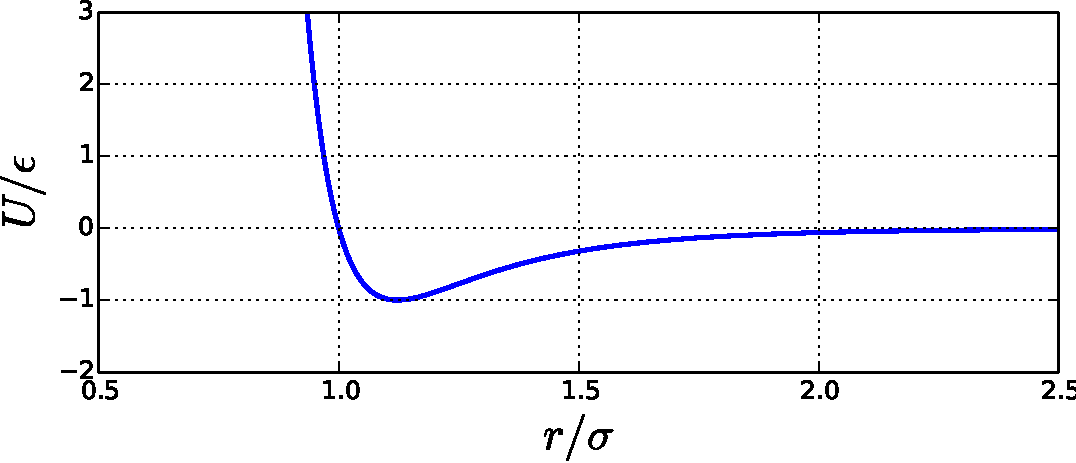
\includegraphics[width=0.75\textwidth]{1}
\end{center}

This potential is of course very simple, but it is perfect for illustrating MD principles, and it works well for idea gases. For more complex MD systems, we can turn to better and more complex potentials such as ReaxFF, there are tons of potentials in the litterature, with enormous varity in complexity and focus. (Weber-Stilling uses normal LJ plus a three-body interaction to describe silicon, the three-body part describes bending stiffness).

\subsubsection*{Integration}

To find the trajectory of the system over time, we must solve the classical equations of motion
$$\frac{\d v}{\d t} = a(t), \qquad \frac{\d x}{\d t} = v(t), \qquad a(t) = \frac{F(t)}{m} = -\frac{\nabla U(r(t))}{m}.$$
Note that these are a set of coupled ODEs, where $v$ describes the velocities of all particles in the system, and $r$ all positions. Now, to solve these, we realize that the derivative of $v$ only depends on the position $r$ and the derivative of $r$ only depends on the velocity $r$, this makes it ideal to solve with a leap-frog scheme. 

However, we would like to avoid the staggered grid of the leap-frog method, so we instead turn to the velocity verlet algorithm. In practice we compute the velocity in two half-steps, we call it a half-kick/draft/half-kick, we have
\begin{align*}
v_{i + 1/2} &= v_i + a_i \frac{\Delta t}{2}, \\
x_{i+1} &= x_i + v_{i+1/2}\Delta t, \\
v_{i + 1} &= v_{i + 1/2} + a_{i+1} \frac{\Delta t}{2}.
\end{align*}
Note that to perform the last step, we have to compute the new acceleration, which includes a force calculation, which is the most expensive part of the calculation. This is why we use velocity-verlet instead of position-verlet.

Just like the leap-frog method, velocity-verlet is a midpoint method integration, and so has global error $\mathcal{O}(\Delta t^2)$. Now, many ODE integration schemes have better accuracy than this (like RK4), so why do we stick to velocity verlet? The main reason is that velocity-verlet is a \emph{symplectic} integrator, which basicly means that it obeys Liovioulle's theorem and preserves the area in phase space. Even though the energy conservation on short time scales will be worse than for a higher-accuracy method like RK4, the long-term stability will be much better for Velocity-verlet due to its symplectic nature. (Other benefits: Preserves time-reversability of the equations of motion. Conserves angular momentum for spherical symmetric potentials, like LJ. Of better order than euler methods, such as Euler-Cromer).

Note that velocity-verlet is \emph{not} energy conserving on short time-scales, which the eq.\ of motions should be. There are higher higher order methods that \emph{are} symplectic, such as the Forest-Ruth algorithm, which is $\mathcal{O}(\Delta t^4$. These methods are usually harder to implement, and require several force calculations per time step, which are expensive. In many simulations, velocity verlet is simply good enough. Other times, we turn to algorithms such as PEFRL. 

\subsubsection*{Cut-off}

The force calculation is expensive as the number of pairs in the system grows as $\mathcal{O}(N^2)$, in comparison, the velcoity-verlet is $\mathcal{O}(N)$ if we disregard the force calculation. However, if we look to our potential, it is obvious that the force between to atoms far away from each other is close to zero, so we can safely ignore these forces in the simulation. We do this by setting a cut-off value, so that $V(r>r_c) = 0$. We should then shift the whole potential up, so that it is still continious in $r_c$.

Any pair of particles that are further away than $r_c$ can now be ignored in our force calculation. Since the particle density is intensive, the force calculation is now of order $\mathcal{O}(N)$. To know which pairs to `skip', we implement neighbor-lists. There are two types: Cell lists and verlet lists. In cell lists, we divide entire system into cells of sides at least $r_c$. For any atom, only atoms in its own cell or neighboring cells can be within $r_c$. We will have to build cell lists for every time step, but this isn't very costly. Verlet lists improve on this, by letting every atom have a list of all other atoms within $r_c + n\eps$. Here we let $\eps$ be of magnitude equal to the max distance an atom can travel in a single time step. We then only have to update the cell and verlet lists every $n$ time steps.

\subsubsection*{Periodic Boundary Conditions}

We need some boundary conditions. There are various posibilities, we could simulate particles in a box (hard walls) or in a vacuum (no walls). These aren't really interesting, as we are often trying to simulate bulk materials, we don't want boundary effects. We therefore use periodic boundary conditions, which are good at simulating a bulk material. If any particle would leave the box, it enters the opposite side of the box with its velocity maintained---this is justified by the concept of \emph{images}, there are many copies of the systems stacked in a regular grid, an atom leaving the system is replaced by a different one entering the opposite end.

To properly evaluate the potential between pairs of particles we need to remember that there are extra images around our system, or we would get the wrong force for atoms close to the boundary. This is implemented by using the `minimum image convention', when calculating the distance between two particles, we need to look for the closest copy of that particle, which doesn't need to be in our box, but could be in the neighboring image. This means the biggest distance between two particles will always be $L/2$ in each dimension.

\subsubsection*{Initialization}

We also need initial condtions. We usually start with out atoms in a regular lattice. In our project we started with all our atoms in a face-centered lattice. This gives a very low potential energy, but it is very safe, as we don't accidently place atoms to close to each other. In addition we give atoms randomly distributed velocities. The distribution is quite forgiving, but we know that the velocities will follow a Boltzmann distribution at equilibrium, so we might as well start them of with such a distribution, we need to eliminate the net drift by subtracting the averege velocity of all particles.

When the system starts it is definitly \emph{not} in thermal equilibrium, due to our regular spacing of atoms. This we will start of with some drastic changes as the system tends to thermal equilibrium, this process is known as \emph{equilibriation} or \emph{thermalization}. We for example expect the velocities of the system to drop rapidly, as the potential energy is very low at the start, and so kinetic energy will be converted to potential energy as the system tends to equilibrium. It is important we let the system really reach equilibrium before we do measurements on the syste, as we only want to study the equilibrium-values.

Since the temperature of the system will change drasticly in the beginning of a simulation, we can use thermostats to prepare a system with a given temperature. After the system has reached the target temperature we must decouple the thermostat if we want to sample the micro-cannonical ensemble, or leave it on to sample the cannonical ensemble.

\subsubsection*{Efficiency improvements}

The cut-off is a hugh efficiency improvement, calculating a big MD system without it is near impossible. In addition we shoul rely on Newton's third law, $F_{ij} = -F_{ji}$ to cut our force-calculation in half. 

MD simulation also lend themselves well to parallelization, we can do it through OpenMP and MPI. This let's us study large MD systems on super-computers.

As always, there are many benefits from smart programming and smart compiling. Use of good C++-features such as inline functions, good use of data-structures, loop unrolling etc, we can get a considerable speed-up.

If we are doing many simulations of similar systems, saving the thermalized state and loading it in might save us a lot of time, instead of having to re-initialize our system for every single simulation.

\clearpage

%%%%%%%%%%%%%%%%%%%%
%%%  QUESTION 2  %%%
%%%%%%%%%%%%%%%%%%%%

\section{MD in the Microcannonical Ensamble}
\begin{itemize}
	\item Discuss initialization and initialization effects
	\item Temperature measurements and fluctuations
	\item Comment on use of thermostats for initialization
\end{itemize}

\subsubsection*{Micro-cannonical ensamble}


An ensemble refers to all possible microstates a system can inhabit under given conditions. In the micro-cannonical ensamble, these conditions are constant number of particles, $N$, volume $V$ and energy $E$. So if we put $N$ atoms in a box of $V$ and let them have total energy $E$, the ensemble are all the possible states these atoms could potentially have---this is obviously an enormous amount of states. 

The \emph{fundamental assumption of statistical mechanics} states that over time, any microstate is equally likely in the isolated system. This let's us calculate thermodynamic properties such as free energy, heat capacity, entropy and so on, at thermal equilibrium, by taking the ensemble average. MD is built on the idea that if we can simulate a system's evolution over time, the trajectory is representative over the entire ensemble. As our system is chaotic, we can be quite sure this is sure. Time averages of our system's trajectory should then be a good approximation to the ensemble average---this is backed up by the ergodic hypothesis.

\subsubsection*{Initialization}

If we want to simulate a system that samples the micro-cannonical ensemble, we must create a system with constant $NVE$. As both $N$ and $V$ are constant, the particle density
$$\rho = \frac{N}{V} = \mbox{constant}.$$
This means we must initialize the system with the right $\rho$ for the phase we want to study, or our result will not be comparable to experiment.

We usually start out system in a regular lattice, such as a FCC lattice. This is because it is quite easiy to implement, and is the structure the system will go to in it's solid phase. It is very safe, as all atoms are even spread out, we avoid having particles being to close to each other. We then start the simulation by giving the atoms all randomly distributed velocities. The distribution we draw the velocities for is quite forgiving, but as we know the system will end up having a Boltzmann distribution at equilibrium, we might as well start them of with such a distribution. After drawing velocities, we subtract any net motion of the system, we interested in internal motion---not center of mass motion.

As we start our system with all atoms in a regular lattice, the system is definitly \emph{not} in thermal equilibrium. And we need to equilibriate the system. The lattice structure means the system has very low potential energy, and a high kinetic energy---over time these will even out, and so the kinetic energy will drop, and the potential energy will increase. This effectively means the temperature of the system will fall. It is important to think of the equilibriation of the system as part of the initialization, as we need to let the system get to equilibrium before we start measuring our time-average, or we will get wrong estimates. 

We see that $N$ and $V$ are easily chosen, $E$ however, is harder. In practice, the easiest way to influence $E$ is by using a thermostat, let us first look at how we measure the temperature.

\clearpage 

\subsubsection*{Temperature measurements and fluctuations}

To measure the temperature of the system, we turn to the equipartition theorem. The equipartition theorem states that at thermal equilibrium, every quadratic degree in the systems Hamiltonian will carry an average energy of $\frac{1}{2}k_b T$. Every atom in our system has three quadratic degrees of freedom in their kinetic energy, so the expectancy of the total kinetic energy of the system will be 
$$\langle E_k \rangle = \frac{3}{2}Nk_bT.$$
In the equipartition theorem, this is the ensemble average of the kinetic energy, but as mentioned, our time-average should be equivalent, so we can consider it the time-average of our system. So we have an estimate to the temperature
$$T = \frac{2\langle E_k \rangle}{3Nk_b}.$$

Now, for the equipartition theorem to be valid, we need to take this average. We could however, define a quantity called the kinetic temperature $T_k$, which is the \emph{instantaenous} temperature
$$T_k = \frac{2 E_k}{3Nk_b},$$
it is important to distinguish between this instantaneous temperature, and the real thermodynamic temperature.

The micro-cannonical ensemble has a constant $NVE$, and within the ensemble we can construct systems with different balances of the potential energy and kinetic energy of the system. This is why we must take an ensemble average of the kinetic energy to get the temperature. Likewise, in our simulation, the total energy is (near) constant, while the total kinetic energy will fluctuate. We thus take the time-averaged kinetic energy. In theory, these fluctuations always take place, but in the thermodynamic limit, where we let $N\to \infty$ and $V\to \infty$ while $\rho$ is held constant, the \emph{relative} fluctuations in the kinetic energy die out, and the temperature will be constant. We then see that temperature $T$ is fundamentally a macroscopic property, and for small systems, $T_k$ will fluctuate much.

\subsubsection*{Thermostats for initialization}

When we are initializing the system, we draw velocities from a Boltzmann distribution with temperature $T_0$, but as we saw, this temperature will \emph{not} be the equilibrium temperature of the system, as a lot of the inital kinetic energy will turn into potential energy before we reach equilibrium. How then, can we study a system prepared to a given target temperature? To do this, we often use a thermostat. A thermostat up- or downregulates the temperature of a system. While a thermostat is working, we are not sampling a micro-cannonical ensamble, since the energy is not held constant. However, we can use a thermostat to bring the system to the target temperature (and thusly energy), and then we can decouple the thermostat, we are now in a micro-cannonical ensemble with the desired energy. 

\clearpage

%%%%%%%%%%%%%%%%%%%%
%%%  QUESTION 3  %%%
%%%%%%%%%%%%%%%%%%%%

\section{MD in the micro-canonical ensemble}
\begin{itemize}
\item How to measure macroscopic quantities, e.g., $T$, $P$, from MD simulation?
\item What challenges do you expect? 
\item What can it be used for?
\end{itemize}

\subsubsection*{Micro-cannonical ensamble}


An ensemble refers to all possible microstates a system can inhabit under given conditions. In the micro-cannonical ensamble, these conditions are constant number of particles, $N$, volume $V$ and energy $E$. So if we put $N$ atoms in a box of $V$ and let them have total energy $E$, the ensemble are all the possible states these atoms could potentially have---this is obviously an enormous amount of states. 

The \emph{fundamental assumption of statistical mechanics} states that over time, any microstate is equally likely in the isolated system. This let's us calculate thermodynamic properties such as free energy, heat capacity, entropy and so on, at thermal equilibrium, by taking the ensemble average. MD is built on the idea that if we can simulate a system's evolution over time, the trajectory is representative over the entire ensemble. As our system is chaotic, we can be quite sure this is sure. Time averages of our system's trajectory should then be a good approximation to the ensemble average---this is backed up by the ergodic hypothesis.

This is then how we measure macroscopic quantities such as temperature and pressure from a MD simulation:
\begin{itemize}
	\item Initialize a system and let it reach equilibrium
	\item Measure the system over long time
	\item The time-average now estimates the ensemble-average
\end{itemize}
Let us look at temperature and pressure as an example. The fundamental quantities we have access to in a simulation is the position and velocity of all particles in the system.

\subsubsection*{Temperature}
To measure the temperature of the system, we turn to the equipartition theorem, which states that at thermal equilibrium, every quadratic degree of freedom in the systems Hamiltonian will carry an average energy of $\frac{1}{2}k_b T$. The velocity of every atom in the system contributes three quadratic degrees of freedom, and so the average kinetic energy at equilibrium should be
$$\langle E_k \rangle = \frac{3}{2}N k_b T,$$
here, the average is an ensemble average. For a micro-cannonical ensemble, the constant quantities are $NVE$, so only the \emph{total} energy is constant, this means the kinetic energy of the various possible microstates will vary. Now, as we know the velocity of every atom in our system, we can easily compute the kinetic energy of our system. Again, the total energy is (nearly) constant, but the kinetic energy will fluctuate. To get a good estimate for the temperature, we should therefore take the time-average.
$$T = \frac{2\langle E_k \rangle}{3Nk_b}.$$

\subsubsection*{Pressure}

In a similar manner, we can estimate the pressure from the virial theorem, we have
$$P = \rho k_b T + \frac{1}{3V}\bigg\langle \sum_{i<j}\vec{F}_{ij} \cdot \vec{r}_{ij} \b\rangle= \rho k_b T + \frac{1}{3V}\b\langle\sum_{i}\vec{F}_{i} \cdot \vec{r}_{i}\b\rangle.$$
The quantity in the expectency is Clausius' virial. As before, this average is an ensemble average, which we can predict from our simulation by taking the time average.

\subsubsection*{Challenges}

In both cases, we see that we need to take the time-average of the quantities. If we \emph{do not} take the time-average, but only look at the instantaneous values of these quantities we have variables that fluctuate quite a lot. The relative size of these fluctuations would die out as the system size increases, and so the definitions of $P$ and $T$ are fundamentally macroscopic, as they are valid in the thermodynamic limit $N\to\infty, V\to \infty, \rho=$ const. At the same time, we can easily calculate and plot the instantaneous values against time and so on. This can be conceptually dangerous.

The main challenge here is that we are measuring a finite system. In the thermodynamic limit we are looking at $N\to \infty$ and $V\to \infty$ in the manner that $\rho = \mbox{const}$. This makes a big difference, as it can be shown that relative fluctations in the system are of order $1/\sqrt{N}$. In the thermodynamic limit, the temperature and pressure are constant and well-defined. In a finite system however, it is not always well-defined, as they are macroscopic quantities.

A challenge for the pressure is measuring the virial in the correct manner, looping over all particles is difficult because of the PBCs and minimum image convention, looping over all pairs seems expensive, but cut-off means that it is only $\mathcal{O}(n)$, and we can do the measurements as we are calculating the force, and so it is actually almost free. We also need to estimate the temperature correctly if want to calculate the pressure.

For the temperature, we must make sure we eliminate any drift in the system, as temperature only corresponds to \emph{internal} motion. We do this when we normalize the system, but if we use a thermostat, it might give the system centre of mass motion, which must then be removed before we try to measure the temperature. There is a numerical artifact called the flying ice cube effect, that is an example of this error, when using a thermostat that messes with the centre of mass motion such as velocity scaling, we might end up with a system that has only drift, and no internal motion, we are thus effectively simulating a frozen cube of ice flying through space.

\subsubsection*{Use of measurements}

\begin{itemize}
	\item Estimate real equilibrium values for real systems. Can for example estimate equation of state, phase transisitons etc.
	\item Gain insight into statistical properties, such as variance of the fluctuations
	\item Study systems that might be hard to study experimentally or under conditions that are hard to do experimentally.
\end{itemize}

\clearpage

%%%%%%%%%%%%%%%%%%%%
%%%  QUESTION 4  %%%
%%%%%%%%%%%%%%%%%%%%

\section{Measuring the diffusion constant in MD simulation}
\begin{itemize}
\item How to measure the diffusion constant in molecular dynamics simulations
\item Limitations and challenges.
\item Compare with methods and results from random walk modeling.
\end{itemize}

\subsubsection*{What is the diffusion constant?}

Diffusion is a measurement of the displacement of individual particles in a system. If there is a concentration gradient in a system, the random motions of individual particles will tend to make the concentration level out and become uniform over time, this phenomena is known as diffusion and is described by Fick's law
$$J = -D\frac{\p \phi}{\p x},$$
where $D$ is the diffusion constant, also known as the diffusion coefficient. It is the proportionality factor between the concentration gradient and the net diffusion flux.

In our molecular dynamics, there is no concentration gradient, and so no net flux. However, there is still \emph{self-diffusion} in the system, meaning individual particles are still moving around in the box, there is a lot of microscopic motion going on. We can focus on the motion of a single particle, it will not have any tendency to move in any given direction, so $\langle r \rangle = 0$, it will however, not tend to be in the same place, so we can find the exepectency of the \emph{mean displacement}: $\langle r^2 \rangle(t)$. 

The macroscopic diffusion is a result of the motion of all the indvidual particles in the gas, it is therefore not strange that you can predict the diffusion. From our study of random walkers, we know that we predict that
$$\langle r^2(t) \rangle \propto 6D t,$$
where the numerical factor of $6$ is only valid in three dimensions, it will be different for other dimensions.

Since our system has a large number of particles, we expect the average mean displacement to be a good estimate of the expectency of a single particle's mean displacement. We can therefore estimate the diffusion constant from the mean square displacement of all particles in the system
$$\langle r^2(t) \rangle = \frac{1}{N}\sum_{i=1^N} (\vec{r}(t) - \vec{r}_{0})^2.$$

By plotting the mean displacement as a function of time, we can use linear regression to find the slope, which is proportional to $D$.

\subsubsection*{Limitations and challenges}

We need to measure the \emph{real} displacement of all particles in the gas, i.e., not use the minimum image convention. We can do this in several ways, we can either keep track of how many times a particle has crossed to the system boundaries. What I did was define the displacement as a 3-vector for every particle. In the velocity-verlet integration algorithm, I updated the displacement in the same manner as the position
$$d_{i+1} = d_i + v_{i+1/2}\Delta t,$$
however, I did \emph{not} enfore the PBCs, and the displacements $d_i$ did not affect the system in any way, unlike the minimum image positions, $r_i$. With this method, we start with $d_i = 0$ as we start measuring the displacement, this way, we don't have to keep track of $r_i(0)$.

We should also simulate the system over long time scales, so we get a better linear fit, which will give a higher precision in the diffusion constant. It is important that the system is thermalized properly before we start measuring the mean square displacement or we will get a wrong estimate of $D$.

For a random walker, we know that
$$\langle r^2(t) \rangle = 6 D t,$$
in 3D, (the numerical constant is 2 in 1D and 4 in 2D). From this we can estimate the diffusion constant. By plotting the measured mean square displacement as a function of time (after the system has been thermalized) we can measure the slope, which will be proportional to the slope.

\subsubsection*{Limitations and challenges}

Should measure the real displacement of the particle, i.e., \emph{not} the minimum image convention. Several ways to do this, keep track of every time a particle moves through a wall. I instead measured the displacement by adding a new varible that was integrated up inside the velocity-verlet. The displacement was not used to calculate any other quantity than the mean displacement.

I was struggling to get a proper $\langle r^2 (t) \rangle \propto t$ behaviour, turns out it was because my initialized temperature was to low, and I was working in a mostly solid phase, meaning there is little to no diffusion.

You also have to initialize the system in the right manner. I was strugling a bit in the beginning, as I thought I had some error in the displacement measurement, turns out I was just trying to measure displacement in a solid phase, which is basicly $D = 0$.

\subsubsection*{Compare to random walker}

A random walker gives insight into diffusion, as it let's us study the motion of a single particle, and then let's us `upscale' the results. A random walker is a particle that has a position that is given as the sum of random increments
$$X_i = \sum_{i=1}^N x_i, \qquad \To \qquad \langle r^2(t) \rangle \propto t.$$
In our projects, we modeled a random walker on a percolating cluster and compared to mean square displacement found in nano-porous flow. There are many parallels we could draw between the two.

\clearpage

%%%%%%%%%%%%%%%%%%%%
%%%  QUESTION 5  %%%
%%%%%%%%%%%%%%%%%%%%


\section{Measuring the radial distribution function in \\ molecular dynamics simulations}
\begin{itemize}
\item How can you measure the radial distribution function in molecular \\ dynamics
simulations.
\item What does it tell?
\item What challenges will you face?
\end{itemize}

\subsubsection*{Definition}

The radial distribution function is the probability density of finding a pair of atoms a distance $r$ away from each other, it is therefore also known as the pair correlation function. If we select an atom in the system as a reference atom, we can also formulate it as the particle density in a spherical shell of radius $r$ from the reference atom. It is usually normalized so that
$$\lim_{r\to \infty} g(r) = 1,$$
which means we must divide the probability by the total particle density of the system, so the local-time-averaged density of a given point a distance $r$ from the reference point is given by $\rho g(r)$.

\subsubsection*{Measuring it in simulation}

The pair correlation function is a probability density of a pair of atoms being a distance $r$ apart. If we then find the distance $r_{ij}$ for every pair of atom in the system, we can bin them into a histogram to estimate the probability density function. Looping over the pair of all atoms and finding the distance between them is already done in the force function, so this is not anything new. We must remember to normalize the bins with respect to the volume of the bins.

\subsubsection*{Use of the pair correlation function}

The pair correlation function can be measured indirectly through neutron and x-ray scattering on a substance. This let's us compare our model to experiments, and verify them.

The pair correlation function tells us something about the average distribution of particles, and thus something about the structure of matter. It will for example be very different for a liquid, a gas and a solid. A solid has a very regular lattice structure, and so the pair correlation function can give us information about this lattice structure.

It turns out that the pair correlation function can be used to predict many macroscopic properties of a substance. Since we find the PCF using microscopic knowledge of the system (the particle positions), the PCF is a bridge from the microscopic to the macroscopic, which is one of the big challenges in molecular dynamics. One such example is Kirkwood-Buff solution theory, which let's us compute thermodynamic qualities from the radial distribution function.

\subsubsection*{What challenges will you face?}

It is not initially obvious what type of binning you should choose. Should you use a linear spacing of $r$-values, or linear in $r^3$ perhaps? It is important to to remember to divide by the correct bin shell volume, and normalize in the correct manner. All these choices depend on each other, so the exact implementation must be consist.

It is of course costly to compute the RDF, as we have to loop over all particle pairs in the system, this is of order $\mathcal{O}(N^2)$, which also gives a large dataset. We might want to do this for many time-steps. A way to reduce this cost is to implement cut-off in a similar manner to the force calculation. We know that $\lim r \to \infty g(r) = 1$, so we might assume that as long as $r > r_{\rm cut}$ we are close enough to 1, and disregard all pairs with distance larger than this. We can then use the cell lists that are already used in the force calculations.

\clearpage

%%%%%%%%%%%%%%%%%%%%
%%%  QUESTION 6  %%%
%%%%%%%%%%%%%%%%%%%%

\section{Thermostats in molecular-dynamics simulations}
Discuss the micro-canonical vs the canonical ensamble in molecular-dynamics
simulations: How can we obtains results from a canonical ensemble? Introduce
two thermostats, and describe their behavior qualitatively. How can you use
such a thermostat for rapid initialization of a micro-canonical simulation?

\clearpage

%%%%%%%%%%%%%%%%%%%%%%%%%%%%%%%%%%%%%%%%%%%%%%%%%%%%%%%%
%%%%%%%%%%%%%%%%%%%%%%%%%%%%%%%%%%%%%%%%%%%%%%%%%%%%%%%%
%%%%%%                                            %%%%%%
%%%%%%        ADVANCED MOLECULAR DYNAMICS         %%%%%%
%%%%%%                                            %%%%%%
%%%%%%%%%%%%%%%%%%%%%%%%%%%%%%%%%%%%%%%%%%%%%%%%%%%%%%%%
%%%%%%%%%%%%%%%%%%%%%%%%%%%%%%%%%%%%%%%%%%%%%%%%%%%%%%%%

%%%%%%%%%%%%%%%%%%%%
%%%  QUESTION 7  %%%
%%%%%%%%%%%%%%%%%%%%

\section{Generating a nanoporous material}
\begin{itemize}
	\item Discuss how we prepare a nanoporous matrix with a given porosity.
	\item How do we characterize the structure of such a material and the dynamics of a fluid in such
a material?
\end{itemize}

\subsubsection*{Generation}
The main idea of MD simulations on nano-porous materials can be summarized in three steps
\begin{enumerate}
	\item First we generate a nano-porous matrix (this is the `solid' material with holes in)
	\item Then we fill the holes with a fluid
	\item Now we do `normal MD simulation' on the fluid, focusing on the measurements connected to our interests. 
\end{enumerate}
A common example is a matrix Silicon dioxide containing water (H$_2$O). This method often looks a lot like the one you would follow if doing experimental physics. You prepare a sample in some manner by manipulating temperatures, strains etc. and once we manage to make a material with the right parameters (porosities etc.), we study it's behaviour. For example one could slowly increase the size of the system while simultaneously cool it.

% In our simulations, a very important functionality is writing the current `state' of our entire system to a file. This is important for visualization, but also because we can then continue a simulation or start a brand new one from the saved state. This way we don't have to initialize and thermalize our system for every single run. 

The way we generated the system in our project is to first simulate a LJ fluid. After the system has thermalized, we `freeze' all atoms in given regions, these atoms will no longer be able to move, and are thus part of a `non-deformable' matrix. They still contribute to the force calculations of the system, but their velocities and positions need not be integrated. The areas not frozen are now the pores in our system, we can remove the atoms in these regions and replace them with an other species, in our project we `replaced' them with a LJ fluid of half-density.

\subsubsection*{Characterization and dynamics}

Characterize the structure of such a material
\begin{itemize}
	\item Porosity $\phi$, the volume ratio of pore space. 
	\item Permeability, $k$. Measure of how easy it is for a fluid to move through the porous material. It is affected by thing such as pore-size, how they are connected and torosity.
\end{itemize}

The simplest characterisitic is the porosity, $\phi$, which is the relative amount of pore space in volume. In my project I simply measured the number of frozen particles and estimated the porosity from the ratio $\phi \approx N_{\rm frozen}/N_{\rm total}$.

To measure the permeability we model flow through the systen. When we model flow there are many interesting 



When filling the pores with a fluid, there are interesting questions that arise---what is the density and pressure of the fluid, do they change with pore size? Can the fluid flow throughout the sample, or are the pores cut off from each other? To characterize the flow, we could for example measure $\langle r^2(t) \rangle$, i.e., the average squared displacement of all fluid atoms in the system as a function of time.

I project 1, we were studying a bulk material, but now we would like to see how pressure is a function of space as well. To do this, we could divide our system into cells, and calculate the pressure in every cell individually, just like we measured the total pressure in the bulk material earlier. If we use the cell lists, we know that only neighboring cells will affect a given cell by a force, and so this will give the correct pressure.

When I measured the average square displacement, I found that it was a linear function with time, just like normal diffusion outside the nano-porous material. I figure this is because the porosity is high enough, and dependant on how the matrix is made. In a system with many small non-connected pores for example, $\langle r(t)^2 \rangle$ would increase at the start of the simulation but should flatten out as all the fluid atoms in a given pore are restricted to move in a small volume.

Lastly we can measure flow of the fluid through the sample by affect all fluid atoms by an external force---think for example of how gravity causes rain to flow down into sand. We use Darcy's law
$$U = \frac{k}{\mu}(\nabla P - \rho g),$$
where $\rho$ is the density, $g$ is the gravitational acceleration. Since $\rho g = Nmg/V$ we replace $\rho g$ with $nF$ where $n$ is the particel density. Darcy law describes the balance between the pressure gradient $\Delta P$ and the external force. The constants $k$ and $\mu$ are the mediums permeability and the fluids viscosity respectively. And $U$ is the volume-flux (i.e., the volume of the fluid that flows through a given cross-section (for example the boundary) for a given time).

Now, from Darcy's law, we can ignore $\nabla P$ in our system, as we don't have hydrostatic conditions, so we have
$$U = -\frac{k}{\mu}nF_x.$$

Now, there are two unknown quantities, so measuring $U$ isn't enough. Now, the permeability $k$ is matrix-dependant and the viscosity $\mu$ is fluid-dependant. We can estimate $\mu$ for a fluid by measuring the velocity profile of flow through a cylindrical pore, which we expect to have the shape
$$u(r) = \frac{\Delta p}{L} \frac{1}{4\mu}(a^2 - r^2).$$
Where $\Delta p$ is the pressure difference (at each end of the cylinder) that leads to flow. For us this is $\Delta p = \rho g \Delta h = nFL$. 

By simulating the flow through a cylinder, at a stationary state (no acceleration), we can now estimate the fluid viscosity, and we can then estimate the permeability for other systems through Darcy's law by measuring the volume flux. Note that the particle density enters into the viscosity, and so it will be different for a high-density and a low-density fluid of the same species. If we are looking at different nanoporous systems we should fill them with a fluid with the same density if we want to use the same viscosity to estimate the permeability!


\clearpage

%%%%%%%%%%%%%%%%%%%%
%%%  QUESTION 8  %%%
%%%%%%%%%%%%%%%%%%%%

\section{Diffusion in a nano-porous material}
\begin{itemize}
\item How can you measure the diffusion constant for a low-density fluid in a nanoporous system? 
\item Discuss what results you expect
\item Compare with bulk liquid and larger-scale porous medium
\end{itemize}

\subsubsection*{The diffusion constant}

Diffusion is a measurement of the displacement of individual particles in a system. If there is a concentration gradient in a system, the random motions of individual particles will tend to make the concentration level out and become uniform over time, this phenomena is known as diffusion and is described by Fick's law
$$J = -D\frac{\p \phi}{\p x},$$
where $D$ is the diffusion constant, also known as the diffusion coefficient. It is the proportionality factor between the concentration gradient and the net diffusion flux.

In our molecular dynamics, there is rarely a concentration gradient, and so no net flux. However, there is still \emph{self-diffusion} in the system, meaning individual particles are still moving around in the box, there is a lot of microscopic motion going on. Predicting the motion of a single atom is difficult, as the microscopic motion is chaotic---we can however talk about the expected motion. For example, most particles won't have a tendency to move in any given direction, so we have $\langle r(t) \rangle = 0$, it will however, tend to not stay in the same place, so we can find the expectancy of the squared displacement: $\langle r^2(t) \rangle$. For a system of many particles, the mean squared displacement will be very close to the expectency, and it turns out that
$$\langle r^2(t) \rangle \propto t.$$
For many systems. In 3D, it turns out that the proportionality constant here is $6D$. We might ask what happens if $\langle r^2 \rangle \not\propto t$, in which case I think Fick's law fails.

From this equation, we can estimate the diffusion constant by measuring the mean displacement of all particles in the system over time, and fitting the result to a linear curve.
$$\langle r^2(t) \rangle = \frac{1}{N}\sum_{i=1^N} (\vec{r}(t) - \vec{r}_{0})^2.$$

This approach works for both bulk liquids as well as porous systems. In a porous system we of course neglect including matrix atoms, we should probably also neglect the particles trapped in pores - as they cannot contribute to macroscopic diffusion, which is what we are actually trying to categorize here.

Since our system has a large number of particles, we expect the average mean displacement to be a good estimate of the expectency of a single particle's mean displacement. We can therefore estimate the diffusion constant from the mean square displacement of all particles in the system
$$\langle r^2(t) \rangle = \frac{1}{N}\sum_{i=1^N} (\vec{r}(t) - \vec{r}_{0})^2.$$

\subsubsection*{What we expect}

We have gained a lot of intuition about the diffusion in a nano-porous medium from our studies of percolating systems. Depending on the porosity of the material and the size and geometry of the pores, a nano-porous material might have diffusion throughout, or the pores can be closed of from each other.

In any case, we always expect a lower diffusion coefficient in a nano-porous material than in a bulk material. This is rather obvious, as random motions will generally disperse over a larger area if it goes unobstructed, as opposed to having to go through thigh pores, bending geometries on so on. In general we have an \emph{effective} diffusion, which we can write as
$$D_e = \frac{D \eps_t \delta}{\tau},$$
here $\eps_t$ is the \emph{transport-available} porosity, which means the ratio of the system which is available for macroscopic transport---i.e., the total volume of the system, minus the solid matrix, minus pores that are too small, minus dead-ends and blind pores (pores not connected to the rest of the pore system). The transport-available porosity is like the backbone in the percolating system. 

We also have $\delta$, which is the constrictivity. In a nano-porous medium, the pores are small, this means that there is a large contribution from surface-effects along the walls. This leads to increasing viscosity, as it is rough for fluid to move along a wall. The constrictivty is a function of the pore size and size of the diffusing particles. The constrictivity is a dimensionless scaling parameter, which is always less than unity: $\delta \leq 1$, a porous medium always has lower diffusion than bulk liquid.

And finally we have $\tau$, the \emph{tortuosity}, which is a mathematical properity a curve can have, that characterized how many turns it has. It is always larger than unity $\tau > 1$. For a porous system with many turns, the mass transport will be lowered, this is described by $\tau$ being larger than 1. We see that all three effects indepdentanly lower the effective diffusion.

\subsubsection*{Compare with diffusion in a bulk liquid and in larger-scale porous medium}

To summarize. In all three systems, we expect the system to follow Fick's law of mass transportation, but with a different diffusion coefficient. We also expect the mean square displacement of indivdiual particles in the pore-system to be proportional to time $\langle r^2 (t) \rangle = 6dt$, so we can measure the diffusion coefficient in all systems with the same tools.

The difference is that we expect the diffusion coefficient to be lower for porous mediums than in bulk, as $\eps_t < 1$, $\tau \geq 1$ and $\delta \leq 1$. For nano-porous we expect the diffusion coefficent to be even smaller, even for the same transport porosity, as the constrictivity is much larger $\delta_{np} < \delta_{p}$, we might also expect the torosity to become larger $\tau_{np} > \tau_{p}$.


\clearpage

%%%%%%%%%%%%%%%%%%%%
%%%  QUESTION 9  %%%
%%%%%%%%%%%%%%%%%%%%

\section{Flow in a nano-porous material}
\begin{itemize}
	\item Discuss how to induce flow in a nano-porous material. 
	\item How can you check your model?
	\item Calculate the fluid viscosity and measure the permeability?
	\item What challenges do you expect?
\end{itemize}

We start of by generating a nano-porous material, this is done by many ways---in our project we simulated a Leonnard-Jones system, after the system has thermalized, we `freeze' all the atoms, and cut out the pores following a random distribution of spheres. The atoms in the solid matrix are not allowed to move in our further simulations of the system, but they do contribute to the force calculations. We fill the pores with new particles (in our simulation, we used the same type of particles, but at half the particle density, in more realistic simulations however, we might have solid material like Si$_2$O filled with H$_2$O). The added particles are allowed to move, but as the solid matrix is frozen, and usually of a much higher density, the fluid can only move inside the pores.

\subsubsection*{Inducing and measuring flow}

If the pores form a connected system, particles can move throughout the system, from one end to the other, this leads to the possibility of macroscopic flow through the system. In normal stochastic simulation of a micro-cannonical ensamble, this flow won't happen, as there is no preassure differential in the system. So how can we induce and measure this flow? We impose a global force on the system.

To answer these questions, we turn to Darcy's law, which for example describes how water flows through aquefiers.
$$U = \frac{k}{\mu}(\nabla P - \rho g).$$
Here $U$ is the volume flux of the water, also called discharge, $k$ is the mediums permeability, and $\mu$ is the fluid's viscosity, $\nabla P$ is the pressure gradient and $\rho g$ is the gravitational force on the water. Darcy's law tells us there are two reasons for volume fluxs in the aquefier system. If there is a pressure differential, there will be a tendency for water to flow from high to low pressure. But gravity also forces water to flow downwards into the ground. In nature, this leads to hydrostatic conditions, where $\nabla P = \rho g$.

Now, in our system, we replace gravity with a general external force acting on all particles equally, $\rho g = \frac{N mg}{V} = n F$, where $n$ is the particle density. In our system, we use periodic boundary conditions, so we won't have a build-up of hydrostatic conditions, and we can generally ignore the pressure gradient
$$U = -\frac{k}{\mu}n F_x.$$
Now, we know the particle density $\rho$, and impose the force $F_x$. We measure the discharge $U$, usually through the periodic boundary condition.

\subsubsection*{Calculate the fluid viscosity and measure the permeability}

The challenge is that both the permeability, $k$, and the viscosity, $\rho$ are unknown. To circumvent this, we use results from a known system, in our case we used the velocity profile through a cylindrical pore, which we expect to have the shape
$$u(r) = \frac{\Delta p}{L} \frac{1}{4\mu}(a^2 - r^2),$$
where $\Delta p$ is the pressure difference at each end of the cylinder, which is given by $\delta p = nFL$. We see that the flow is fastest in the center of the cylinder, far away from the walls. Close to the walls, there is little flow. 

We can measure the velocity profile at a stationary state by measuring and binning the results for various $r$ into a histogram. This gives us the velocity profile, and we can estime the viscosity $\mu$. The viscosity is fluid dependant, and we can use this parameter in other nano-porous systems. So we can now estime the permeability $k$ of different nano-porous systems. 

\subsubsection*{Challenges}

We should measure the discharge from Darcy's law and the velocity profile in a cylindrical pore at a stationary state (no net acceleration), it is therefore important to let our simulation run long enough before sampling.

We should also be a little careful with transfering the viscosity of a fluid. For one, it depends non-trivially on the particle density $n$, so we should only use it for various NPSs if we maintain a relatively equal particle density.

\clearpage

%%%%%%%%%%%%%%%%%%%%%%%%%%%%%%%%%%%%%%%%%%%%%%%%%%%%%%%%
%%%%%%%%%%%%%%%%%%%%%%%%%%%%%%%%%%%%%%%%%%%%%%%%%%%%%%%%
%%%%%%                                            %%%%%%
%%%%%%             PERCOLATION                    %%%%%%
%%%%%%                                            %%%%%%
%%%%%%%%%%%%%%%%%%%%%%%%%%%%%%%%%%%%%%%%%%%%%%%%%%%%%%%%
%%%%%%%%%%%%%%%%%%%%%%%%%%%%%%%%%%%%%%%%%%%%%%%%%%%%%%%%

%%%%%%%%%%%%%%%%%%%%
%%%  QUESTION 10 %%%
%%%%%%%%%%%%%%%%%%%%

\section{Algorithms for percolation systems}
\begin{itemize}
\item How do we generate a percolation system for simulations? 
\item How to analyze and visualize the systems?
\item How to find spanning clusters and measure the percolation probability?
\end{itemize}

\subsubsection*{Generate}

We choose some geometry in some dimension, we have usually been studying a $L\times L$ 2D grid. We then let every `site' in the geometry be either occupied with probability $p$, or unoccupied with probability $1-p$. To do this, we draw a random number from $[0, 1)$ for every site (uncorrelated) and check this value against $p$. Every site with a random number less than $p$ is occupied. This is done very quickly in matlab/python, which creates a random matrix and checks it against some threshold very simple. 

\subsubsection*{Analyze and visualize}

We now have our system, which is some matrix of 0's and 1's. We now choose some neighbor-system, we have been working with only closest neighbors (4 neighbors in 2D, not diagonal). Any occpuied site `in direct contact', meaning you can step from one to the other going only through occupied sites, belong to the same cluster. Our job is thus to go through the matrix, and find all the different clusters. Every cluster is given a unique number label. This can be done quite simply
\begin{enumerate}
	\item Loop over entire matrix. 
	\item Skip all unoccupied sites and occpuied sites that have already recieved a label
	\item If you hit an occupied site that has no label, label it with current label counter and check for neighbors without labels.
	\item If you find a neighbor without label, goto (3). Else: Increase label counter
\end{enumerate}
In practice both matlab and python have good tools built in to do this, \verb+bwlabel+ and \verb+measurements.label+ respepctively.

Once we have all the labels, we plot the matrix, and give each cluster it's own color. We can either choose color based on cluster-size, or randomize it completely. We should however, \emph{not}, color according to label number. The labeling algorithm cause the label number to increase in a steady fashion, so clusters close together get similar label numbers. In most practical cases, we will get very many clusters, and so the color difference between them will be very small, thus to nearly equal labels will give a color that is almost impossible to tell apart.

We can find the area/mass of any cluster my counting the number of times a given label occurs in the label-matrix.

To find a spanning cluster, we first identify the paired boundaries of our system (often left-right or top-bottom or both). We then find the sets of all labels that occur on either boundary independantly, and intersect the two sets. If a label exist on both boundaries, that cluster is by definition a spanning cluster. For square matrixes, we can also find the minimum bounding box, and checking the width/height against the width/height of the system, matlab and python both have automatic tools for finding bounding boxes of the cluster.

\subsubsection*{Percolation probability}

The percolation probability, $\Pi(p,L)$ gives the probability that a system is percolating. 

If we generate a single matrix and check if it is percolating, we of course find that it either is, or it isn't. So if we generate $N$ such systems (same $p$, same $L$) we find that $n$ of them are percolating, then the ratio $n/N$ approximates $\Pi(p,L)$. For good statistics, we want $N$ to be as high as possible. 

We can of course repeat this for many $(p, L)$ sets to find how the function varies as a function of $p$ and $L$.


\clearpage

%%%%%%%%%%%%%%%%%%%%
%%%  QUESTION 11 %%%
%%%%%%%%%%%%%%%%%%%%

\section{Percolation on small lattices}
\begin{itemize}
	\item Discuss the percolation problem on a $2\times 2$ lattice.
	\item Sketch $P(p, L)$ and $\Pi(p, L)$ for small $L$.
	\item Relate to your simulations.
	\item How do you calculate these quantities and how do you measure them in simulations?
\end{itemize}

   

\subsubsection*{Introduction}

We want to find the percolation probability $\Pi(p, L)$ and the spanning cluster density $P(p, L)$ for a $L\times L$ matrix. For small $L$ we can just write out all the possible configurations, write up the probability of them all, and compute the probabilities $\Pi$ and $P$ on closed form. However, the possible number of configurations grows exponentially with the system size $2^{L\times L}$, however, the insight gained from the small $L$ is very valuable, so let us start by studying a $2\times 2$ and end by relating this to numerical results for higher $L$.


\subsubsection*{All configurations}
We use nearest neighbor connectivity and consider both left-right and top-bottom to be spanning. There are $2^4 = 16$ possible configurations. We write them all out below:

\begin{center}
$1\times$
\begin{tabular}{|c|c|}
  \hline
  \ \ \ &  \ \ \  \\ \hline
  \qquad & \qquad \\
  \hline
\end{tabular} \qquad
\qquad $4\times$
\begin{tabular}{|c|c|}
  \hline
  \ \ \cellcolor{black} &  \ \ \  \\ \hline
  \ \ \ & \qquad \\
  \hline
\end{tabular} \qquad 
\qquad $2\times$
\begin{tabular}{|c|c|}
  \hline
  \ \ \ & \cellcolor{black} \ \ \  \\ \hline
  \cellcolor{black} & \qquad \\
  \hline
\end{tabular}	

$4\times$
\begin{tabular}{|c|c|}
  \hline
  \ \ \cellcolor{black}&  \ \ \  \\ \hline
  \ \ \cellcolor{black} & \qquad \\
  \hline
\end{tabular} \qquad
\qquad $4\times$
\begin{tabular}{|c|c|}
  \hline
  \  \cellcolor{black} & \cellcolor{black} \ \ \  \\ \hline
  \ \  \cellcolor{black} & \qquad \\
  \hline
\end{tabular} \qquad 
\qquad $1\times$
\begin{tabular}{|c|c|}
  \hline
  \ \ \cellcolor{black} & \cellcolor{black} \ \ \  \\ \hline
  \cellcolor{black} & \cellcolor{black} \qquad \\
  \hline
\end{tabular}	
\end{center}
The probability of any given configuration is given by $p^x(1-p)^{4-x}$ where $x$ is the number of occupied clusters. This gives the expressions
\begin{align*}
\Pi(p, L) &= 4p^2(1-p)^2 + 4p^3(1-p) + p^4, \\
P(p, L) &= 2\cdot 4p^2(1-p)^2 + 3\cdot 4p^3(1-p) + 4\cdot p^4. \\
\end{align*}
A plot is shown at the start of the next page 
\begin{figure}[ht]
\centering
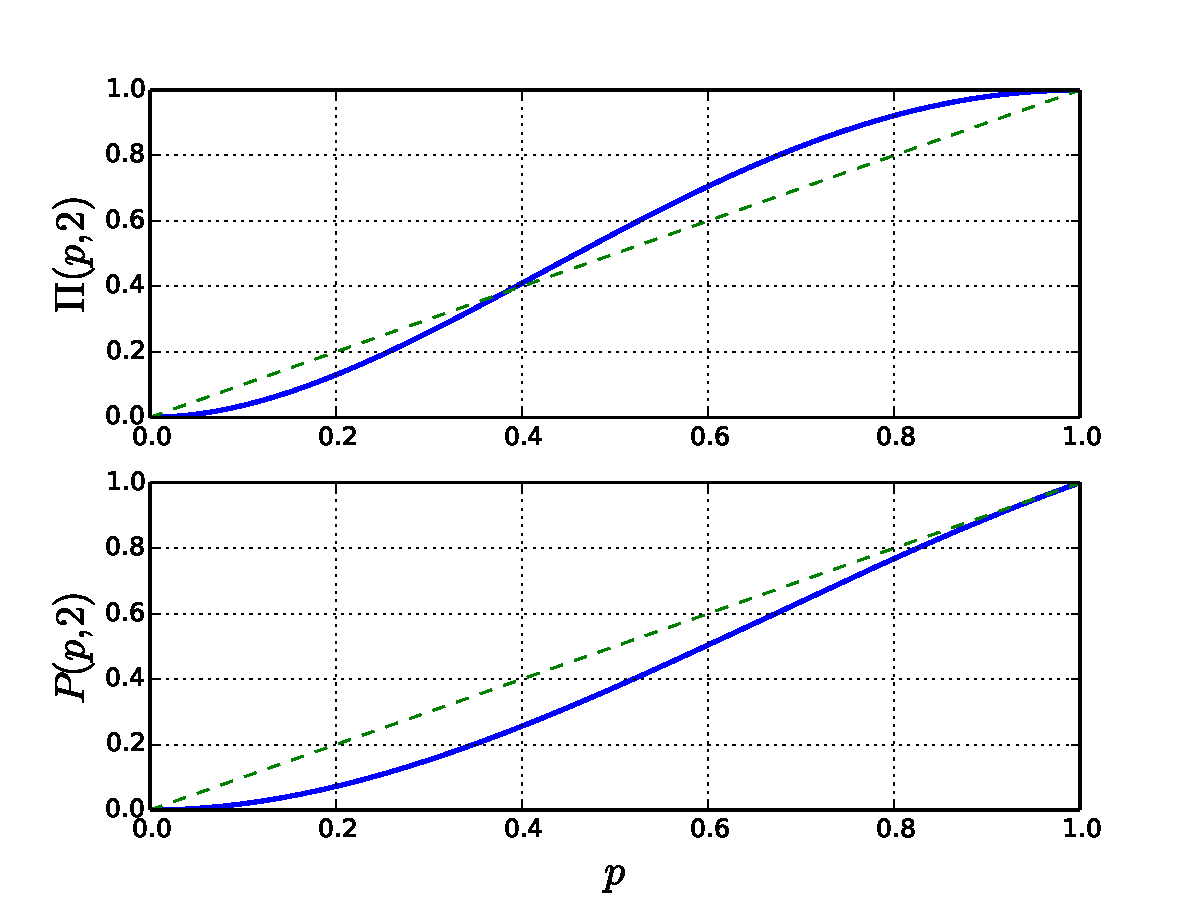
\includegraphics[width=\textwidth]{11.pdf}
\end{figure}

\newpage
We note some things about the curves: Both curves start at $0$ for $p=0$ and go to $1$ as $p\to 1$, this is very intuitive. They are also completely smooth. Note that the spanning cluster density is always below $p$, this makes perfect sense. The spanning cluster density is the probability of a random site to be a part of the spanning cluster. Now, the random site doesn't \emph{have} to be occupied, so the highest-estimate for $P$ should always be $p$---and occupied sites don't have to be part of a spanning cluster. In this case, if there \emph{is} a spanning cluster, all occupied sites automatically belong to it, so it is not surprising that the the difference from $p$ dies out as $\Pi\to 1$. For larger clusters however, it is very possible to have both a spanning cluster, and non-spanning cluster in the same experiment.

\subsection*{Measuring $\Pi(p,L)$ and $P(p, L)$ numerically}

For larger lattices, listing all the possible configurations becomes impossible due to the sheer number of them. Instead we do monte carlo simulations. By generating $N$ matrices of size $L$ and checking them against the probability $p$, we can look at the number of them that are percolating, the ratio of percolating systems to the total number of systems simulated gives an estimate for $\Pi(p,L)$ that improves as $N$ improves.

\clearpage

%%%%%%%%%%%%%%%%%%%%
%%%  QUESTION 12 %%%
%%%%%%%%%%%%%%%%%%%%

\section{ Cluster number density in 1-d percolation}
\begin{itemize}
	\item Define the cluster number density for 1-d percolation
	\item Show how it can be measured.
	\item Discuss the behavior when $p \to p_c$. How does it relate to your simulations in two-dimensional systems?
\end{itemize}

\subsubsection*{Definition of number cluster density}

In a random system, there will usually be very many different clusters of varying shapes and sizes. When $p > p_c$ there will usually be one or more spanning clusters, but also many non-spanning clusters. When $p < p_c$ there will usually just be many non-spanning clusters. We might ask the question how the sizes of the clusters are distributed, and how that distribution changes as $p \to p_c$. When $p\to p_c$ the clusters will tend to rapidly grow larger untill they become the system size and the system becomes percolating. The cluster number density $n(s,p)$ is part of this distribution

\paragraph{Definition} 
The cluster number density is the probability for a random site in the matrix to be a specific site in a cluster of size $s$.

The normalization requirement on the number cluster density is
$$P + \sum_s s n(s,p) = p,$$
In 1D, $p_c = 1$ so $P = 0$ when $p<p_c$ and we get
$$\sum_s s n(s,p) = (1-p)^2 p \sum_s s p^{s-1} =  (1-p^2) \frac{\d}{\d p} \sum_s p^s = (1-p^2) p \frac{\d}{\d p} (1-p^2)^{-1} = p.$$


The probability for a random site to be part of a cluster of size $s$ is then $sn(s,p)$, since any cluster of size $s$ has $s$ specific sites. In 1D, for a site to be the left-most site in a cluster of size $L$ is given by the fact that we need $p$ occupied sites and 2 non-occupied sites surrounding those $s$ sites.
$$n(s,p) = p^s (1-p)^2.$$
because a random site has a probability $p$ to be occupied, and then it is either part of the spanning cluster, or of a non-spanning cluster of size $s$. 

\subsubsection*{Characteristic cluster size}
To get a better understangin of $n(s,p)$, let us consider $p$ to be a constant. And look at the $s$-dependance of $n(s,p)$. In this case, $(1-p)^2$ is basicly just a normalization constant, and of no interest, so we look at only 
$$G(s) = n(s,p)(1-p)^{-2} = p^s.$$
If we plot a log-log plot of this function against $s$, we get 
\begin{figure}[ht]
\centering
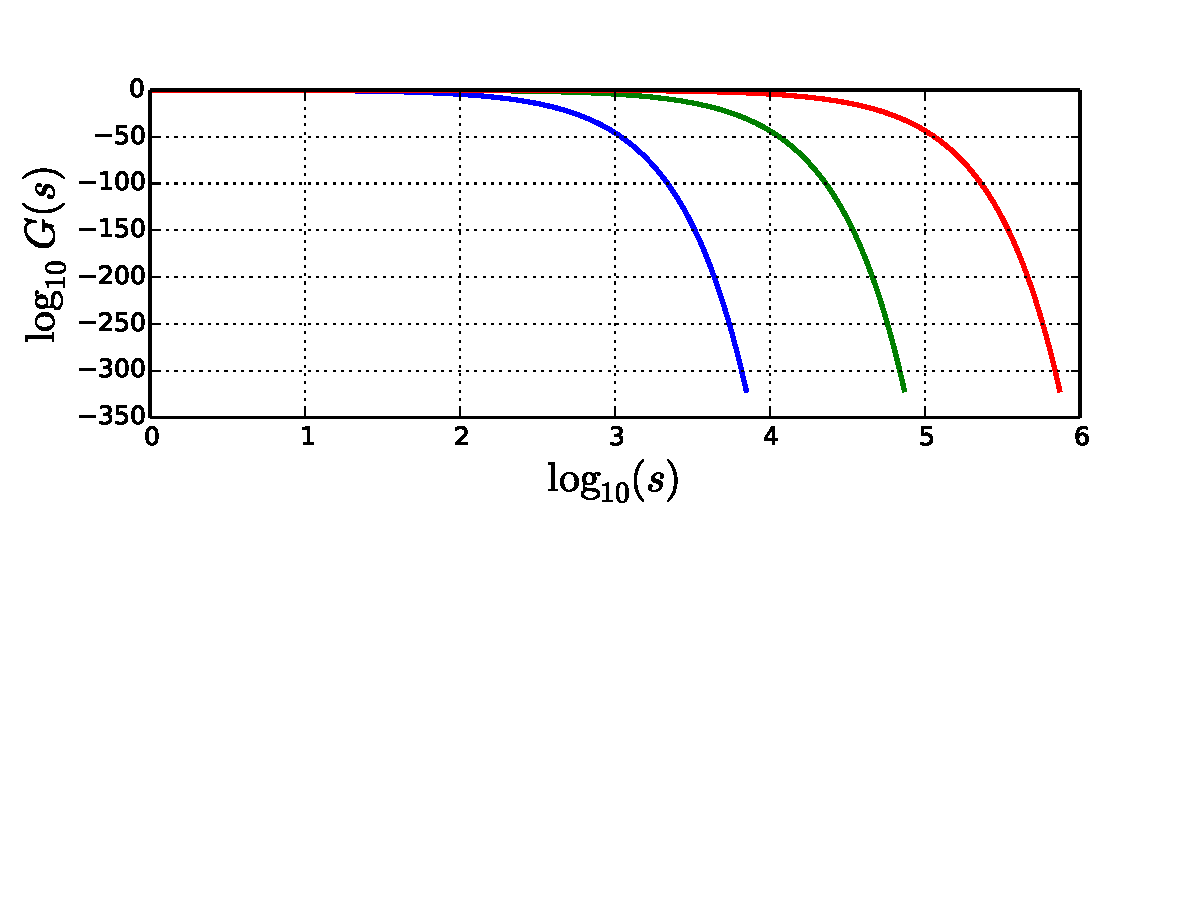
\includegraphics[width=\textwidth]{12.pdf}
\end{figure}
To understand this function we rewrite $G$ as follows
$$G(s) = p^s = e^{s \ln p} = e^{-s/s_\xi}, \qquad s_\xi \equiv -\frac{1}{\ln p}.$$
Where $s_\xi$ is the cut-off cluster size, also referred to as the characteristic cluster size. It is a cut-off, as 
$$G(s) = e^{-s/s_\xi} = \begin{cases}
1 & s \ll s_\xi, \\
0 & s \gg s_\xi, \\
\end{cases},$$
so when $s\to s_\xi$, $G$ (and thereby $n(s,p)$) starts decay exponentially.

\subsubsection*{Dependence on $p$}
We see that the $p$-dependence enters as $p$ affects how large the characteristic cluster size is
$$s_\xi = -\frac{1}{\ln p},$$
from this, we see that $s_\xi$ grows with $p$ (in 1D), which is very intuitive. As $p\to p_c (= 1)$ we can Taylor-expand
$$-\frac{1}{\ln p} = -\frac{1}{\ln(1 - (1 - p))} \simeq \frac{1}{1-p}.$$
And as $1 = p_c$ we get
$$s_\xi \simeq \frac{1}{p_c-p} = |p-p_c|^{-1/\sigma}.$$
Which is the general form of $s_\xi$ in \emph{any} dimension. In 1D, $\sigma = 1$.

So as $p\to p_c$, $s_\xi$ diverges as a power law.

\paragraph{Data collapse:} As the only $p$-dependence of $n(s,p)$ enters through $s_\xi$, we expect a data collapse if we instead plot $G$ as a function of $s/s_\xi$. To include the normalization $(1-p)^2$ we use the Taylor expansion, so that $(1-p)^2 \simeq s_\xi^{-2}$. So that we get
$$n(s,p) = s^{-\tau} F\bigg(\frac{s}{s_\xi}\bigg).$$

\subsubsection*{Numerical simulation}

We can generate a system with threshold $p$, and then count the number of clusters of size $s$: $N_s$ (the spanning cluster should not be included!). We can then estimate the cluster number density from
$$\bar{n(s,p)} = \frac{N_S}{L^d}.$$
A better estimate would of course be given by doing many experiments
$$\bar{n(s,p)} = \frac{N_S(M)}{ML^d}.$$
To do the counting $N_S(M)$ in a meaningful manner, we should use logarithmic binning as we have a fat tail.

\clearpage

%%%%%%%%%%%%%%%%%%%%
%%%  QUESTION 13 %%%
%%%%%%%%%%%%%%%%%%%%

\section{Correlation length in 1-d percolation}
\begin{itemize}
	\item Define the correlation length $\xi$ for 1-d percolation.
	\item Discuss its behavior when $p \to p_c$. 
	\item How is it related to cluster geometry and your results for twodimensional percolation?	
\end{itemize}

\subsubsection*{Correlation length $\xi$}

The characteristic cluster size $s_\xi$ says something about the size/mass/area of a cluster. The correlation length however, is used to characterize the extent of a cluster. We first define the correlation function $g(r)$, which is the probability of two occupied sites being a distance $r$ apart of begin connected---the $r$ coordinate is an integer denoting the number sites in between. In 1D, this is quite simple to compute, it is simply
$$g(r) = p^r = e^{r \ln p} = e^{-r/\xi}.$$
This function is quite flat for low $r$, but as $r\to \xi$ it starts to die out very fast. We see from the definition of $\xi$ that it diverges as $p\to 1$, this is due to the fact that $1 = p_c$. We use that fact that $p \to 1$ to Taylor expand
$$\ln p \sim -(1-p),$$
so we find that correlation length diverges as a power law
$$\xi = (1-p)^{-1}.$$

For a general dimensional system, it can be shown that
$$\xi = \xi_0(p_c - p)^{-\nu},$$
so $\xi$ diverges as a power law when $p \to p_c$.

\subsubsection*{Cluster geometry}

Now, the characteristic length says something about the extent of the cluster, but what about it's geometry? We can define a variance for the geometry of the cluster, such a quantitiy is known as the \emph{radius of gyration}. We define it as
$$R_i^2 = \frac{1}{s_i}\sum_{n=1}^{s_i} (\vec{r}_i - \vec{R}_i)^2.$$
Where $R_i$ is the radius of gyration for a given cluster $i$, $s_i$ is the cluster size, $n$ is a site label, $\vec{r}$ is the site location and $\vec{R}_i$ is the clusters centre of mass.

\subsubsection*{2D percolation}
For 1D, the extent and mass of a cluster is the same thing (a cluster can't be hollow), so 
$$s_\xi = \xi, \qquad \mbox{characteriztic cluster size = correlation length}$$
however, in higher dimensions
$$s_\xi \propto \xi^D, \qquad \mbox{where } D \mbox{ is a fractal dimensionality constant } D < d.$$


An intersting use for $\xi$ is that it tells us when a finite system size will be a good approximation to an infite lattice. As we have done numerical modeling of a 2D lattice (it is not analytically solvable), we must neccesarily have a finite $L$, which might affect our results dramatically. However, if $\xi \ll L$, there should be no clusters of extent close to the lattice size, as the clusters of size larger than $\xi$ are exponentially surpressed. However, if $\xi \gg L$ there's a high probability of clusters the size of the system, and so the finite system size will definitely affect the results. As $\xi$ diverges as $p\to p_c$, a finite system size $L$ will never be a truely good approximation to the infite cluster as $p \to p_c$. 

We have
\begin{align*}
s_\xi &\propto |p-p_c|^{-1/\sigma}, \\
s_\xi &\propto \xi^D = |p-p_c|^{-D\nu}, \\
D\nu\sigma &= 1.
\end{align*}

\begin{center}
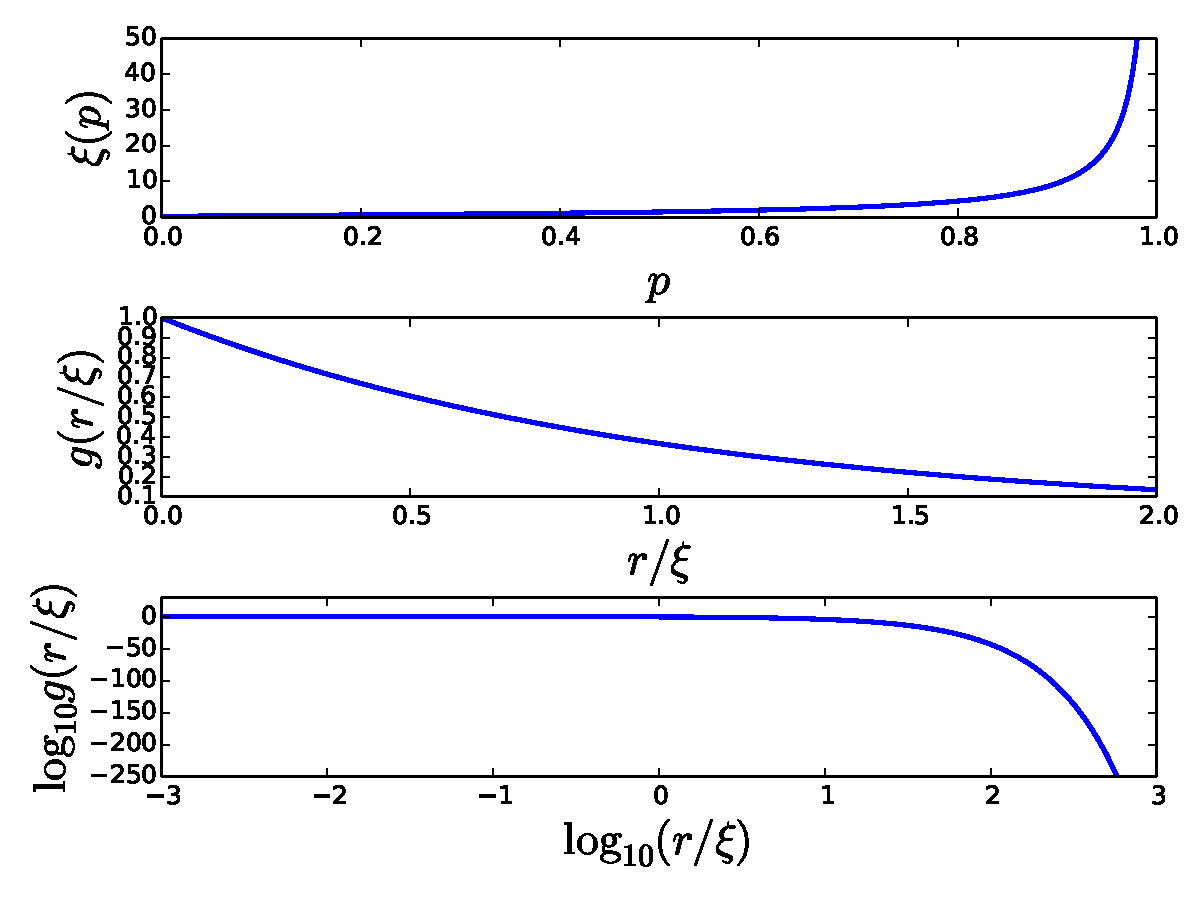
\includegraphics[width=0.8\textwidth]{13.pdf}
\end{center}


\clearpage

%%%%%%%%%%%%%%%%%%%%
%%%  QUESTION 14 %%%
%%%%%%%%%%%%%%%%%%%%

\section{Cluster size in 1-d percolation}
\begin{itemize}
	\item Introduce the characteristic cluster size for the 1-d percolation problem.
	\item Discuss their behavior when $p \to p_c$.
	\item Relate to your simuluations on 2-d percolation.
\end{itemize}


A random system will have clusters of varying shapes and sizes. In 1D percolation, all clusters of the same size look the same. The cluster number density is the probability for a given site to be a specific site of a cluster of size $s$, so the probability density of cluster sizes is given by
$$sn(s,p).$$
If we focus only on the cluster number density, in 1D it becomes
$$n(s,p) = (1-p)^2 p^s.$$
Now, the $(1-p)^2$ is constant for a constant $p$, so it isn't that important, but we have
$$p^s = e^{s \ln p} = e^{-s/s_\xi}, \qquad s_\xi = -1/\ln p,$$
and this is the characteristic cluster size $s_\xi$. Not that $n(s,p)$ is pretty constant when $s < s_\xi$ but that it quickly dies out when $s > s_\xi$. It doesn't matter that the probability of a given site to be occupied is multiplied by $s$, as $n(s,p)$ dies out exponentially when $s > s_\xi$, and $s$ only grows linearily.

So the characteristic cluster size is the biggest cluster size it is reasonable to find in our random system.

\subsubsection*{When $p \to p_c$}
Now, let's study the definition of $s_\xi$
$$s_\xi = -\frac{1}{\ln p}, \qquad p\in [0,1] \To s_\xi \in [0, \infty].$$
So the characteristic cluster sizes diverges when $p \to 1$. The reason for this is that $p_c=1$ for the 1D system. So that as $p\to 1$ we are expecting bigger and bigger clusters to form, but as long as $p = 1-\eps$ for a finite  $\eps$, the infinite 1D cluster hasn't started percolating.

\subsubsection*{Comparison with 2D}

In 2D, the characteristic cluster size talks about the total \emph{mass} of clusters, that means, the total number of sites in the cluster. It does not take into account the shape or geometry of the cluster. In 1D we found that the characteristic cluster size diverges as a power law as $p\to p_c$, this same behaviour is observed in 2D, but with a different power constant
$$s_\xi = |p-p_c|^{-1/\sigma}.$$
(Note that $\sigma < 1$, so the characteristic cluster size diverges \emph{faster} in 2D). The reason for divergence is exactly the same in 2D. As long as $p < p_c$, there is no spanning cluster, but as $p$ is getting very close, we are getting very large, but still \emph{finite}, clusters. As $p=p_c$, the system starts percolating and forms a spanning cluster, meaning $s_\xi$ `reached' infity. As $p > p_c$ we see an exact reversed trend, where $s_\xi$ goes back down, this is because the characteristic cluster size is connected to the cluster number density and is only used to describe the fintie (non-spanning) clusters, so as $p > p_c$ and $p$ increases, the added probability causes the spanning cluster to grow in size, and it `swallows' other finite clusters. The bigger a finite cluster is, the bigger the probability of it being swallowed by the spanning cluster, so it makes sense that $s_\xi$ decreasing as a power law. As $p \to 1$, we should obviously have $s_\xi \to 0$ as the probability of any finite clusters is 0. So we see that the power law doesn't hold, but this isn't surprising as the power law is only valid when $|p-p_c|$ is small, we used a Taylor expansion to first order.

\clearpage

%%%%%%%%%%%%%%%%%%%%
%%%  QUESTION 15 %%%
%%%%%%%%%%%%%%%%%%%%


\section{Measurement and behavior of $P(p, L)$ and $\Pi(p, L)$}
\begin{itemize}
\item Discuss the behavior of $P(p, L)$ and $\Pi(p, L)$ in a system with a finite system
size $L$.
\item How do you measure these quantities?
\end{itemize}

\subsubsection*{Definition}

The percolation probability $\Pi(p, L)$ is the probability of a random system of size $L$ to have at least 1 spanning cluster, when every site is inhibited with probability $p$. The spanning cluster density $P(p,L)$ is the probability a given site has of being a part of the spanning cluster, it is called the spanning cluster density, because it is equal to the average spanning cluster mass divied by the number of sites in the system. A system of `size' $L$ is different in 1D and 2D.

\subsubsection*{The behaviour of $P(p, L)$ and $\Pi(p, L)$}

Let us start at $L=\infty$. When the system is infite in size, there is a given value $p_c$ where the system will always start to percolate. In 1D it is obvious that $p_c = 1$, since a single unihabited site will prevent a spanning cluster from forming. In 2D it is $p_c = 0.59275$. The percolation probablity $\Pi(p,L)$ is then simply a step function at $p=p_c$.  For the other extreme, $L=1$, the 1D and 2D cases are the same, and we get the linear curve $\Pi(p, 1) = p$ in both cases. 
\begin{center}
	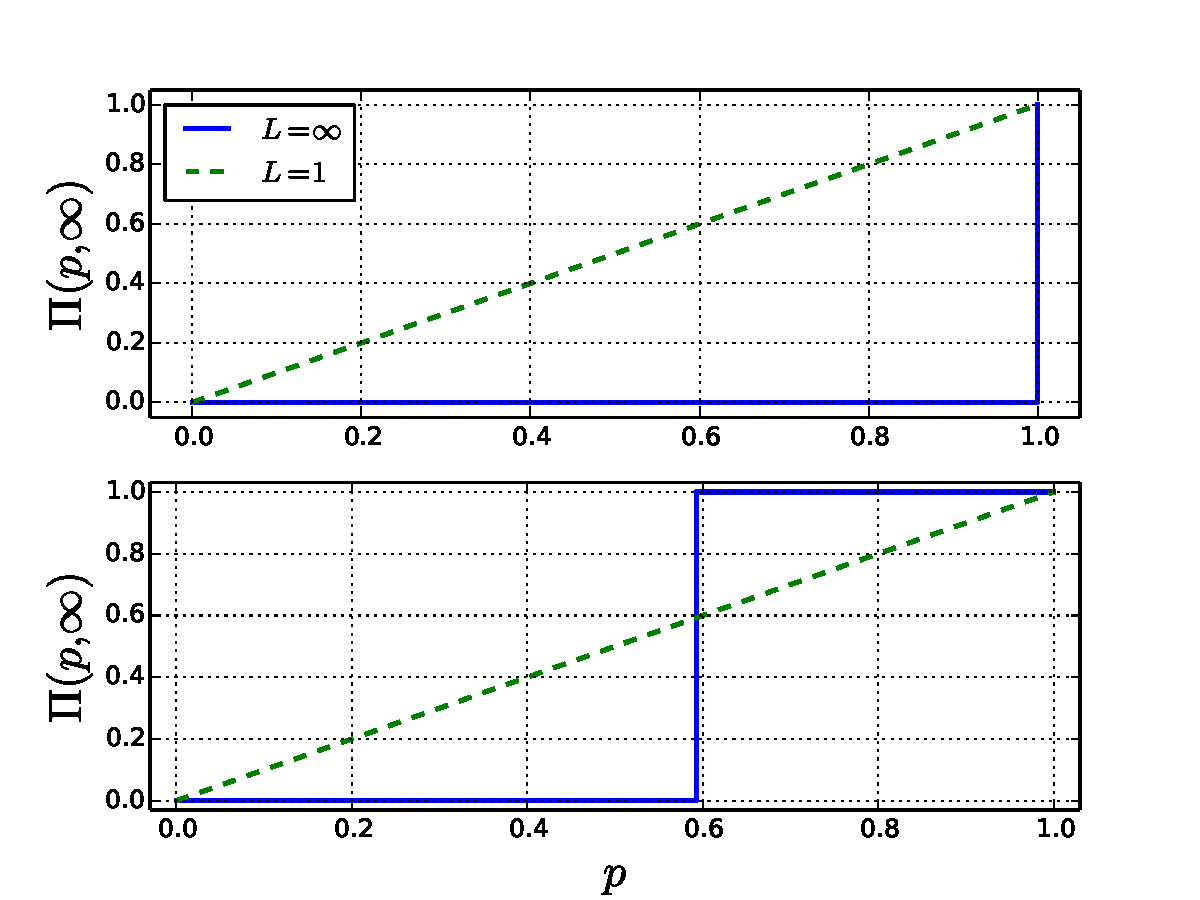
\includegraphics[width=0.7\textwidth]{15.pdf}
\end{center}

Now, let us look at small, but finite $L$. In 1D, the probability is easy to find
$$\Pi(p,L) = p^L,$$
And we see that as $L$ grows, it quickly dies out for small $L$. When $p \to 1$ the probability goes to 1, the bigger the system, the steeper this slope is. So the probability is a monotonely decreasing function as $L$ grows. This is very intuitive: for the system to be percolating, we have to `get lucky' and get every site occupied. For a small $L$ this is very doable, but as $L$ grows, it becomes impossible. You can throw a 5-dice yahtzee, but you can't throw a million-dice yahtzee.

\begin{center}
	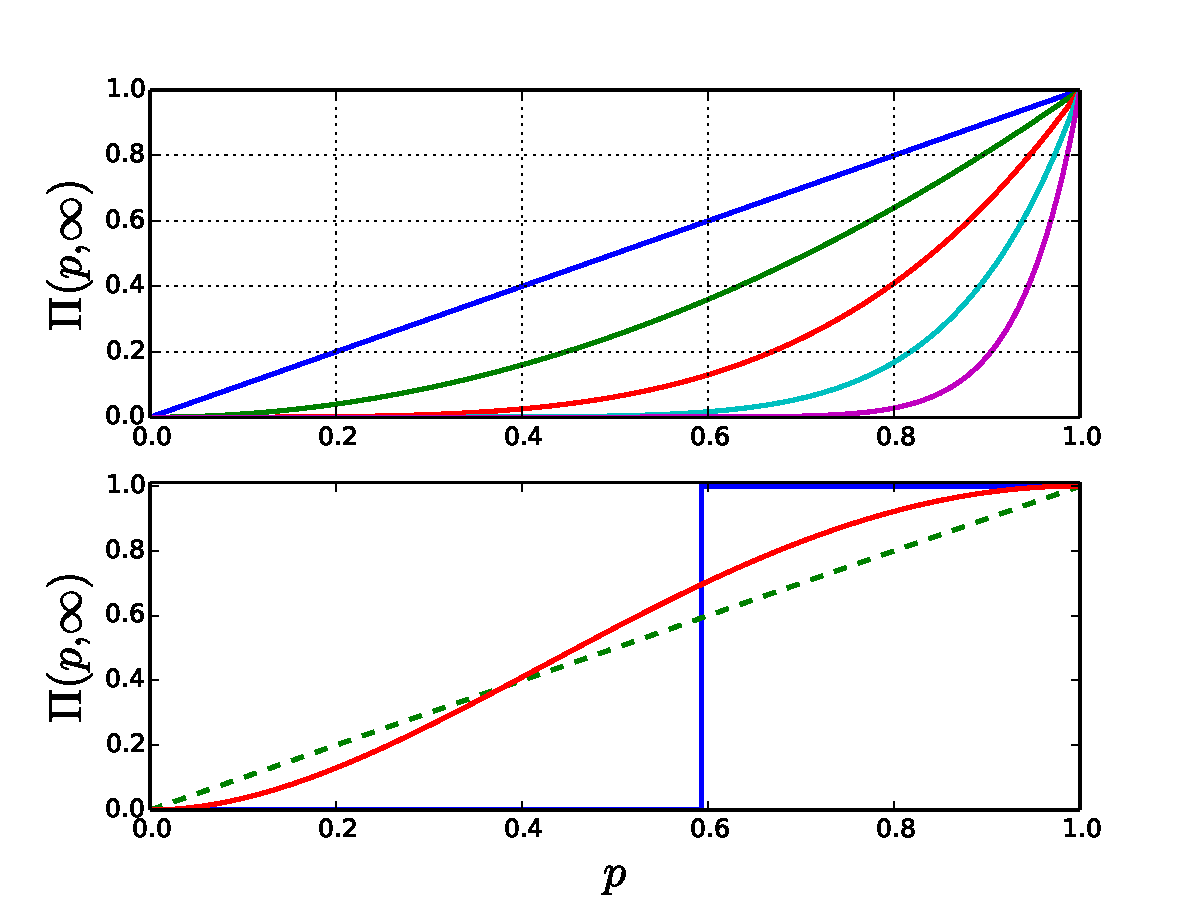
\includegraphics[width=0.7\textwidth]{15b.pdf}
\end{center}

For 2D, there is no easy expression for the percolation probability as function of $L$, but for the smallest $L$ we can tabulate all possible configurations, weight them according to their probabilities, and then find the expection value for the percolation probability by summing over them (and their weights). The number of configurations grows as $2^{L\times L}$, so it grows exponentially with the system size. Let us quickly show $L=2$ as an example, there are 16 configurations, of these, 9 are percolating

\begin{center}
$4\times$
\begin{tabular}{|c|c|}
  \hline
  \ \ \cellcolor{black}&  \ \ \  \\ \hline
  \ \ \cellcolor{black} & \qquad \\
  \hline
\end{tabular} \qquad
\qquad $4\times$
\begin{tabular}{|c|c|}
  \hline
  \  \cellcolor{black} & \cellcolor{black} \ \ \  \\ \hline
  \ \  \cellcolor{black} & \qquad \\
  \hline
\end{tabular} \qquad 
\qquad $1\times$
\begin{tabular}{|c|c|}
  \hline
  \ \ \cellcolor{black} & \cellcolor{black} \ \ \  \\ \hline
  \cellcolor{black} & \cellcolor{black} \qquad \\
  \hline
\end{tabular}	
\end{center}
So from this we get
$$\Pi(p, 2) = 4p^2(1-p)^2 + 4p^3(1-p) + p^4, \\$$

We see that close to $p=0$ and $p=1$, the function is starting to `glue' to the correct $P=0$. As we increase $L$, we see this trend continues, giving a sharper and sharper slope. We can interpret this phenomena much like that for 1D. In the infinite lattice, we need $p=p_c$ to percolate, and we will always percolate above $p_c$. In a finite lattice however, we can get `lucky', and just happen to get a percolation cluster at $p \leq p_c$, just like for 1D, in 2D however, we can also be `unlucky', in that we might not have a spanning cluster even for $p > p_c$. As $L$ grows, the chance of being `lucky' and `unlucky' both become smaller and smaller, and in the $L\to \infty$ limit, we cannot be either lucky or unlucky anymore, we have the step function.


\subsubsection*{Measurement}

The idea to find $\Pi(p, L)$ for small $L$ was to list all configurations and then find the expected value by taking the sum of configurations weighted by their probabilities. For big $L$, this isn't possible, since there are two many possible configurations. However, if we create a random matrix, this is the same as sampling configuration space, drawing out a configuration at random. If we draw out $N$ samples, and $N_p$ of them are percolating, we can then estimate the percolation probability from
$$\Pi(p, L) \simeq \frac{N_p}{N}.$$

To create a random matrix, we draw a $L\times L$ matrix of random numbers uniformly distributed in $[0,1]$. Then we check every site against the preset $p$, any site with value less than $p$ is inhabited, every site with value more than $p$ is not inhabited.
 

\clearpage

%%%%%%%%%%%%%%%%%%%%
%%%  QUESTION 16 %%%
%%%%%%%%%%%%%%%%%%%%

\section{The cluster number density}
Introduce the cluster number density and its applications: 
\begin{itemize}
	\item Definition
	\item Measurement
	\item Scaling
	\item Data-collapse
\end{itemize}

\subsubsection*{Definition}

The cluster number density is the probability of a random site being a specific site in a cluster of size $s$. It will have the normalization condition
$$\sum_s sn(s,p) + P(p) = p,$$
because any site is either not occupied $(1-p)$, part of the spanning cluster $P$, or part of a finite-sized cluster $n(s,p)$.

\subsubsection*{Measurement}

We generate a $L\times L$ matrix, and make every site be occupied with probability $p$ (uncorrelated between sites). After generating the matrix, we can label all clusters, and find their masses. This is done automatically in matlab using the \emph{regionprops.Area}-command, but it is quite easy to do. Once we have all clusters and their masses (we do \emph{not} include the spanning cluster), we can estimate the cluster number density from 
$$\overline{n(s,p)} = \frac{N_S}{L^{d}},$$
where $N_S$ is the number of clusters of site $S$. Usually we want to do this many times, to get better data, so we generate $M$ such systems, and keep track of the
 running total of clusters of size $s$.
$$\overline{n(s,p)} = \frac{N_S(M)}{ML^{d}}.$$

Now, there are very many different possible values of $s$, so we want to use binning, Meaning we combine results for close-lying $s$-values. This gives us a histogram that estimates the probability density $n(s,p)$. However, it turns out $n(s,p)$ is a probability density with a fat tail, meaning large $s$-values are not very likely, but more likely than in a expoential distribution (so called Black Swan behaviour of power laws). If we use uniform bin sizes, this means we will have very many bins without any hits in them! To solve this problem, we use logarithmic binning, meaning we let the bins grow in size as we get larger and larger $s$-values, in an exponential fashion. When using non-uniform bin sizes, we must remember to divide by the correct bin size to get the right probability density in the end, or the tail ends of the probability density would become exponentially overexposed.

\subsubsection*{Scaling}
To describe the scaling of the cluster number density, let us consider the 1D case, where we have
$$n(s,p) = (1-p)^2 p^s = G(s)(1-p)^2.$$
Now, for a given $p$ value, the $(1-p)^2$ factor is just a constant, so let us look at the $G(s)$ function, it is given as
$$G(s) = p^s = e^{s \ln p} = e^{-s/s_\xi}, \qquad s_\xi = -\frac{1}{\ln p}.$$
Here we have introduced the characteristic cluster size, $s_\xi$. We see that $G(s)$ is quite constant when $s \ll s_\xi$, but when $s > s_\xi$ it decays exponentially, and so it is effectively 0 as soon as $s \gg s_\xi$. This means for a given system, we do not expect to find any clusters much larger than $s_\xi$.

Now, let us see what happens when $p$ grows. As $p\in[0,1]$, we find that $s_\xi = -1/\ln p \in (0, \infty)$, and so as $p$ grows, $s_\xi$ grows. In a log-log plot of $G(s)$ vs $s$ we will se a very flat function, untill we hit $s_\xi$, when it falls off.
\begin{figure}[ht]
\centering
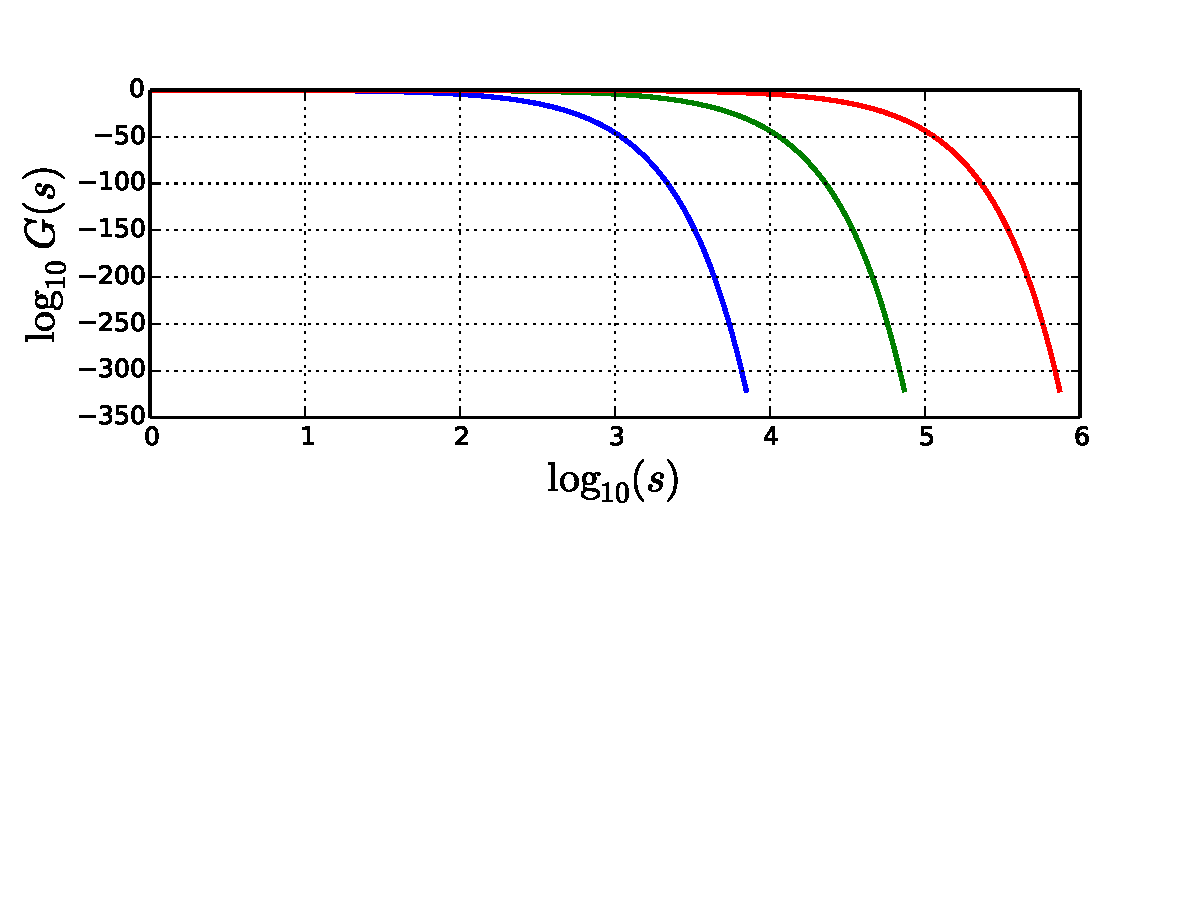
\includegraphics[width=\textwidth]{12.pdf}
\end{figure}

\vspace{-4cm}

Now, for $p\to 1$, $s_\xi \to \infty$, so the characteristic cluster size diverges, this can be shown from $-1/\ln p = 1/(1-p)$, so we have
$$s_\xi = (1-p)^{-1}.$$
This phenomenon is true for any dimension, where $s_\xi$ diverges as $p\to p_c$,
$$s_\xi = |p-p_c|^{-1/\sigma}.$$

Now, why does $s_\xi$ diverge. It is because as $p\to p_c$ we are getting close to a spanning cluster (infinite in size), but we aren't quite there yet. When $p$ crosses over, so $p > p_c$, there is a spanning cluster, and the characteristic cluster size falls down as a power law again, as the spanning cluster starts `eating' the larger clusters in the system.

\subsubsection*{Data-collapse}

We see that $G(s)$ looked different for various $p$-values. This is because there is a $p$-dependence through $s_\xi$. We can get rid of the $s_\xi$ dependence by plotting $G(s/s_\xi)$ instead. In that case, all the curves move on top of each other. This is what is known as a \emph{data-collapse}. If we have a numerical data-set, or something gotten from experiments, we can plot our data as a function of $s/s_\xi$, and we then know that our results should have no $p$-dependence, all the datasets should collapse into 1, there will be some small differences due to noise, but if there are any large deviations---we know there must be some systematic error in our experiment.

Now, the cluster number density was given by
$$n(s,p) = G(s)(1-p)^2.$$
Now, plotting this as a function of $s_\xi$ does not lead to data collapse, due to the normalization factor, but we can fix this by using the approximation of the logarithm close to $p_c$, so that $(1-p)^2 = s_\xi^{-2}$, so we have
$$n(s,p) = G(s) \bigg(\frac{s}{s_\xi}\bigg) s^{-2} = s^{-2} F\bigg(\frac{s}{s_\xi}\bigg).$$
The behaviour is general for all dimensions, but the factor 2 changes
$$n(s,p) = s^{-\tau} F\bigg(\frac{s}{s_\xi}\bigg).$$
Here $F$ act's as the cut-off function. When we plot $F$ as a function $s/s_\xi$ we predict a data-collapse.

\clearpage

%%%%%%%%%%%%%%%%%%%%
%%%  QUESTION 17 %%%
%%%%%%%%%%%%%%%%%%%%

\section{Finite size scaling of $\Pi(p, L)$}
\begin{itemize}
	\item Discuss the behavior of $\Pi(p, L)$ in a system with a finite system size $L$.
	\item How can we use this to find the scaling exponent $\nu$
	\item And the percolation threshold, $p_c$?
\end{itemize}

In numerical simulations, we are force to work with a finite $L$, but we want to find results for an `infite' lattice size. To study how the finite size lattice differs from the infite lattice, we use finite size scaling. We have a correlation length, which diverges as a power law when $p \to p_c$:
$$\xi \propto |p-p_c|^{-\nu}.$$

The correlation length describes what the largest extent of a cluster we expect in our system is. It is very unlikely to find a cluster with extent much larger than $\xi$. The correlation length gives a good indication of when the finite size of the system is important. If $\xi \ll L$, we don't expect any cluster close to the system size, and so the cluster won't `see' the finite size lattice. If $\xi \gg L$ we expect at least a few clusters of size close to the system size, and so the finite size of the system definitly affects our results. If we think of our system as a slice of a larger (or even infite system), the $\xi \gg L$ case means we have cut the biggest clusters up by slicing out our system. While for $\xi \ll L$ we might slice some clusters on the boundary, but the clusters in the middle of our lattice have been untouched.

As $\xi$ diverges when $p \to p_c$, which is usually the $p$-range we are most interested in studying, it is obvious that our finite lattice size often will be problematic. Finitie size scaling let's us describe the effects of the finite size system.


When $\xi \gg L$, the system will appear to be on the percolation treshold, even though the infite lattice might not even be close. When $\xi \ll L$ however, the system seems homogeneous at lengths longer than $\xi$.

We want to study the thermodynamic limit ($L\to \infty$) of a quantity $X(p)$ that acts as a power law when $p\to p_c$. Examples are $P(p)$, $S(p)$ and $M(p)$.

We have
$$X(p) \propto (p-p_c)^{-\gamma_x}.$$
The finite size scaling ansatz is
$$X(p, L) = L^{\frac{\gamma x}{\nu}} \chi \bigg(\frac{L}{\xi}\bigg).$$

Our approach is always to assume that the finite size scaling problems will always be to assume that the finite size enters through a scaling function modyfining the asymptotic behavior, that is, we assume
$$P(p, L) = (p-p_c)^\beta X\bigg(\frac{L}{\xi}\bigg).$$
For $L \gg \xi$ we require $P$ to require the thermodynamic limit behaviour ($L\to \infty$), so we require that $X(u) = 1$ for $u \gg 1$. When we are in the finite size limit however, $\xi \ll L$, we expect the system to only depend on the system size $L$, since we `cut' out the systems knowledge of $\xi$.
$$P(p, L) = (p - p_c)^\beta X \bigg(\frac{L}{\xi}\bigg) = \xi^{-\beta / \nu} X\bigg(\frac{L}{\xi}\bigg) = Y(L).$$
Where we have used 
$$\xi = \xi_0(p-p_c)^{-\nu}.$$

Now, we need $P$ to be independant of $\xi$, so $X(L/\xi)$ must have a $\xi^{-\beta/\nu}$ proportionality. So we have
$$X(u) = \begin{cases}
	constant & \mbox{when } u\gg1 \\
	u^{-\beta/\nu} & \mbox{when } u\ll1.
\end{cases}$$
And so from this we find that
$$P(p,L) = \begin{cases}
	\xi^{-\beta/\nu} & \mbox{for } L \gg \xi \\
	L ^{-\beta/\nu} & \mbox{for } L \ll \xi. 
\end{cases}.$$

\subsubsection*{Behaviour of $\Pi(p, L)$}
In the thermodynamic limit, the percolation probability is a step-function at $p=p_c$. For lower $L$, it is more `smeared' out. If we consider how it is affected by the finite size of the lattice, it makes sense that 
$$\Pi(p, L) = \begin{cases}
	1 & \mbox{for } \xi \gg L \\
	0 & \mbox{for } \xi \ll L.
\end{cases}$$
In any case, it is obvious that it really should be a function of $L/\eps$, so we have
$$\Pi(p, L) = f\bigg(\frac{L}{\xi}\bigg).$$
In 1d, we can find this function analytically, and it is simply $\Pi(p, L) = p^s = e^{-L/\xi}$. In 2D we can't find it analytically, but we don't need the exact form, just the fact that it is a function of the $L/\xi$ ratio is enough. We write
$$\Pi(p, L) = f\bigg(\frac{L}{\xi_0(p-p_c)^{-\nu}}\bigg) = \tilde{f}\big(L(p-p_c)^{\nu}\big) = \Phi\big((p-p_x)L^{1/\nu}\big).$$

Now we flip the question slightly, and say, if we want the percolation probability to be a specific number, let's say 60 \%, what does $p$ need to be? This of course varies with $L$, so we have
$$\Pi(p_{\pi=x}(L), L) = x.$$
Inserting our expression for $\Pi$ gives
$$\Phi\big((p_{\pi=x}-p_c L^{1/\nu}\big) = x.$$
Now, we don't know the exact form of $\Phi$, but we know it is a smooth function that goes from 1 to 0, so we know our inverse exists for our $x$, so we get
$$(p-p_c L^{1/\nu} = \Phi^{-1}(x).$$
The inverse of $x$ will just be some constant $C_x$, it generally depends on our choice of $x$, but \emph{not} on $L$, that is the important part
$$(p_{\Pi=x}-p_c) L^{1/\nu} = \Phi^{-1}(x).$$
Now we have
$$p_{\Pi=x}(L) = p_c + C_x L^{-1/\nu}.$$

Now, from this expression, we measure $p_{\Pi=x}(L)$ numerically, we do not know $p_c$, $C_x$ or $\nu$. So how do we proceed. Well, let us measure for $x_1$ and $x_2$ and study the difference
$$\Delta p(L) = p_{\Pi=x_1}(L) - p_{\Pi=x_1}(L) = (C_{x_1} - C_{x_2}) L^{-1/\nu} = AL^{-1/\nu}.$$
To measure something useful from this, we plot $\log \Delta p$ against $\log L$, 
$$\log \Delta p(L) = -\frac{1}{\nu}\log L + \log A,$$
from this we see that this should be a linear function with slope $-1/\nu$. Using linear regression on our dataset gives us an estimate for $\nu$.

We now turn back to 
$$p_{\Pi=x}(L) = p_c + C_x L^{-1/\nu}.$$
For a given dataset we plot $p_{\Pi=x}(L)$ against $L^{-1/\nu}$, we see that this gives a straight line with slope $C_x$ and intersect $p_c$. Another linear regression lets us find $p_c$.




\clearpage

%%%%%%%%%%%%%%%%%%%%
%%%  QUESTION 18 %%%
%%%%%%%%%%%%%%%%%%%%

\section{ Subsets of the spanning cluster}
\begin{itemize}
	\item Introduce and discuss the scaling of subsets of the spanning cluster.
	\item How can we measure the singly-connected bonds, and how does it scale?
\end{itemize}

\subsubsection*{Subsets of the spanning cluster}

In a percolating system of size $L$, we can envision flow through the spanning cluster. When looking at this flow, we can characterize each site belonging to the spanning cluster in three ways
\begin{itemize}
	\item The singly connected bonds 
	\item The backbone
	\item The dangling ends
\end{itemize}

The singly connected bonds are sites that, if they were removed, the spanning cluster would cease to be spanning. If we think of the flow through a spanning cluster, the singly-connected bonds are bottlenecks, and so all the fluid \emph{must} pass through any given SCD before making it's way through the system. 

The backbone of the system are any site in the spanning cluster than have more than one path leading into them, one from either side of the cluster. If we study flow through the spanning cluster, the backbone will be the part of the system accesible to the flow. Note that the SCBs are part of the backbone!

The dangling ends are the parts of the spanning cluster than only have one site leading into them. If this site is removed, we cut of the dangling end. Any flow into a dangling end will have nowhere to go, and so the dangling ends will have no flow if we apply a pressure to the system, they are `dead ends'.

\subsubsection*{Scaling}

We might wonder what ratio of the spanning cluster that compromises the SCDs, the backbone and the DEs respectively. And also how this changes with system size. We know that the mass of the spanning cluster itself follows a power law
$$M \propto L^D, \qquad D \leq d$$
Where the parameter $D$ is referred to as the fractal dimension of the spanning cluster. It is obvious that $D \leq d$ is the true dimensionaly of the system. If $p=1$, the mass of the spanning cluster grows as $M = L^d$ with the system size, if $p<1$, then it is obvious that the mass of the spanning cluster grows slower than the total number of sites in the lattice as any added site would on average contribute $p$ cluster mass, which might go into a finite cluster.

We now propose that the mass of all singly connect bonds, all backbone and all dangling ends all individually follow similar power laws, but with different fractal dimensions
\begin{align*}
	M_{\rm SC} &\propto L^{D_{\rm SC}}, \\
	M_{\rm BB} &\propto L^{D_{\rm BB}}, \\
	M_{\rm DE} &\propto L^{D_{\rm DE}},
\end{align*}
or compactly
$$M_i \propto L^{D_i}, \qquad i \in \{\mbox{SCD}, \mbox{BB}, \mbox{DE}\}.$$

Since all three sets are subsets of the spanning cluster, we must have that 
$$D_i \leq D, \qquad i \in \{\mbox{SCD}, \mbox{BB}, \mbox{DE}\}.$$

\subsubsection*{Measurement}

If we are doing numerical simulations, we need some algorithm to find the SCBs, the BB and the dangling ends of a system. We can do this by using self-avoiding random walks on the spanning cluster. We can start SAWs started at either end of the spanning cluster. The intersect of all SAWs that make it to the other end of the system will be the SCBs, as any path through the system must go through the SCBs. The backbone is the union of all SAWs that make it through the cluster, as the backbone are the sites accesible to flow. Lastely, if we take the union of all SAWs that do \emph{not} make it through the system, and subtract the backbone, we find the dangling ends. In effect, the SAWs enter a dangling end, and get trapped.

As the SCBs are given by the intersect of all SAWs, it cannot grow faster than the minium SAW length through the system, which grows as
$$L_{\rm min} = L^{D_{\rm min}},$$
this must mean that
$$D_{\rm SC} \leq D_{\rm min}.$$
Likewise, the backbone is given by the union of all SAW path that make it through the system, so it must grow at least as fast as the maximum SAW path that makes it through, so
$$D_{\rm BB} \ge D_{\rm max}.$$

We have the following hierarchy
$$D_{\rm SC} \leq D_{\rm min} \leq D_{\rm SAW} \leq D_{\rm max} \leq D_{BB} \leq D \leq d.$$
The only missing dimensionality are the dangling ends. All we can say for certain is that we must have
$$D_{\rm DE} \leq D.$$
and 
$$D_{\rm BB} \leq D.$$
But we cannot have $D_{\rm DE} < D$ and $D_{\rm BB} < D$ at the same time, as this would lead to
$$aL^{D_{\rm DE}} + bL^{D_{\rm BB}} = cL^D,$$
Dividing by $L^D$ and taking the limit $L \to \infty$ would give
$$c = 0.$$

We can estimate the dimensionalities by counting the masses at $p=p_c$. Another approach is using renormalization group method.

One can use renormalization theory to make theoretical arguments about the fractal dimensionality. At $p=p_c$ the spanning cluster is a self-fractal.

Theoretical value: $D_{SC} = 1/\nu = 3/4$.

In our project 3, I didn't use SAWs to find SCDs, BBs and DEs, I am guessing this is computationally costly if we need all possible SAW paths, not sure though. We were given a script that calculated a flow through the spanning cluster by solving Kirchoff's law (The net flux into a given site has to be zero, if it weren't fluid would accumulate in a site). After finding the flux through a site, we can characterize any site in the spanning cluster as follows
\begin{itemize}
	\item No flow? $\to$ Dangling end
	\item Some flow? $\to$ Backbone
	\item Max flow? $\to$ Singly-connected bond
\end{itemize}


\clearpage

%%%%%%%%%%%%%%%%%%%%
%%%  QUESTION 19 %%%
%%%%%%%%%%%%%%%%%%%%

\section{ Random walks / Flow in a disordered system}
\begin{itemize}
	\item[Either:] Discuss the scaling theory for the distance $r^2(t)$ of a random walker
dropped at a random occopied site on either (1) the percolation system or (2)
the spanning cluster. (You can choose which case to discuss). Relate the results
to diffusion in a bulk fluid and in a nanoporous system.
\item[Or: ] How do you measure the conductivity of the spanning cluster? Discuss the
scaling theory for the conductivity $\sigma(p, L)$
\end{itemize}

\clearpage

\section*{Appendix}

\subsubsection*{Box-Muller transform}

The Box-Muller transform is a way to convert randomly drawn numbers from $[0,1)$ to standard normally distributed numbers. There are two versions of the Box-Muller transform, the basic and the polar. Both versions draw to independant uniformely random numbers, $u$ and $v$ from $(0,1)$ and generate two normal numbers at once using trigonometric functions. The difference is that the polar form implements rejection sampling. If the random numbers $u$ and $v$ are such $u^2 + v^2 \geq 1$, we reject the pair and draw two new ones. Initially this seems inefficient, (we need roughly 1.3 input numbers per output number) but the computation from $u$ and $v$ to normal numbers is computationally cheaper and for most modern computers trigonometric functions are much more expensive than drawing rand numbers.

\section*{Questions}

Are the signs in Darcy's Law as given in project 2 opposite? Look at wikipedia. Why would the volume flux be \emph{opposite} of the applied force? The law now says that flow goes \emph{against} the pressure gradient (from low pressure to high pressure).

When applying a global force to our system, why doesn't the energy of the system increse indefinitly? The particles affected by the global force are accelerating, and we have no energy flow out of the system, no?


If we lock $L$ and vary $p$, we can use the same underlying matrix and check it versus different $p$ values, we can then find the $p'$ value that makes that exact matrix percolate. Is this a better approach than generating a new random matrix for each $p$? Why/why not? 

\section*{Nice formulations}

\subsubsection*{Microcanonical ensemble $NVE$}
\begin{itemize}
	\item System is isolated
	\item Total energy is fixed, constant $E$
	\item Every accesible microstate is equiprobable, so $\Omega$ is multiplicity, 
	$$P(s) = \frac{\Omega(s)}{\sum_s \Omega(s)}.$$
	\item Satisfies ergodicity, time averages can be replaced with ensemble averages.
\end{itemize}

\subsubsection*{Canonical ensemble $NVT$}
\begin{itemize}
	\item System is not isolated. Can exchange energy with a heat bath. Total energy of heat bath + system is constant. The equilibrium energy of the system is constant
	\item The equilibrium $T$ is fixed, but it will fluctuate.
	\item Probabilities in the system are given by Boltzmann distribution
	\item Approaches the microcannonical ensemble in the thermodynamic limit, as relative fluctuations go as $\propto 1/\sqrt{N}$.
\end{itemize}

Why do we use cannonical ensemble? It is easier to study cannonical ensemble than isolated ensemble in experiments. It also guarantees stability in the energy.

Fluctuations in pressure are not a worry, the only worry is that the pressure we are simulating at is far to low or far to high, we must be sure that our particle densitiy is what we want it to be at at the start of the simulation.



\end{document}



 
